\documentclass{book}
\usepackage[a4paper,top=2.5cm,bottom=2.5cm,left=2.5cm,right=2.5cm]{geometry}
\usepackage{makeidx}
\usepackage{natbib}
\usepackage{graphicx}
\usepackage{multicol}
\usepackage{float}
\usepackage{listings}
\usepackage{color}
\usepackage{ifthen}
\usepackage[table]{xcolor}
\usepackage{textcomp}
\usepackage{alltt}
\usepackage{ifpdf}
\ifpdf
\usepackage[pdftex,
            pagebackref=true,
            colorlinks=true,
            linkcolor=blue,
            unicode
           ]{hyperref}
\else
\usepackage[ps2pdf,
            pagebackref=true,
            colorlinks=true,
            linkcolor=blue,
            unicode
           ]{hyperref}
\usepackage{pspicture}
\fi
\usepackage[utf8]{inputenc}
\usepackage[french]{babel}

\usepackage{mathptmx}
\usepackage[scaled=.90]{helvet}
\usepackage{courier}
\usepackage{sectsty}
\usepackage{amssymb}
\usepackage[titles]{tocloft}
\usepackage{doxygen}
\lstset{language=C++,inputencoding=utf8,basicstyle=\footnotesize,breaklines=true,breakatwhitespace=true,tabsize=8,numbers=left }
\makeindex
\setcounter{tocdepth}{3}
\renewcommand{\footrulewidth}{0.4pt}
\renewcommand{\familydefault}{\sfdefault}
\hfuzz=15pt
\setlength{\emergencystretch}{15pt}
\hbadness=750
\tolerance=750
\begin{document}
\hypersetup{pageanchor=false,citecolor=blue}
\begin{titlepage}
\vspace*{7cm}
\begin{center}
{\Large Dictionnaire \\[1ex]\large 1.\-0 }\\
\vspace*{1cm}
{\large Généré par Doxygen 1.8.1.2}\\
\vspace*{0.5cm}
{\small Vendredi Avril 25 2014 01:05:38}\\
\end{center}
\end{titlepage}
\clearemptydoublepage
\pagenumbering{roman}
\tableofcontents
\clearemptydoublepage
\pagenumbering{arabic}
\hypersetup{pageanchor=true,citecolor=blue}
\chapter{Liste des éléments obsolètes}
\label{deprecated}
\hypertarget{deprecated}{}

\begin{DoxyRefList}
\item[\label{deprecated__deprecated000001}%
\hypertarget{deprecated__deprecated000001}{}%
Membre \hyperlink{classabstract__dictionnaire_a0b04fb9d2062846f5c9bdc8c7742538f}{abstract\-\_\-dictionnaire$<$ V $>$\-:\-:to\-\_\-array} () const =0]utiliser to\-\_\-list()  
\item[\label{deprecated__deprecated000002}%
\hypertarget{deprecated__deprecated000002}{}%
Membre \hyperlink{classhash__dictionnaire_a4ea9ee40aa51412199f64a6dce55842d}{hash\-\_\-dictionnaire$<$ V, S $>$\-:\-:to\-\_\-array} () const ]utiliser to\-\_\-list()  
\item[\label{deprecated__deprecated000003}%
\hypertarget{deprecated__deprecated000003}{}%
Membre \hyperlink{classhash__table_aa65cffb759b4b5f480e71bf59f8268db}{hash\-\_\-table$<$ K, V, S $>$\-:\-:keys\-\_\-array} () const ]utiliser to\-\_\-list()  
\item[\label{deprecated__deprecated000004}%
\hypertarget{deprecated__deprecated000004}{}%
Membre \hyperlink{classhash__table_a8ec288028398a823c9c3450afbf4592f}{hash\-\_\-table$<$ K, V, S $>$\-:\-:values\-\_\-array} () const ]Utiliser to\-\_\-list()  
\item[\label{deprecated__deprecated000005}%
\hypertarget{deprecated__deprecated000005}{}%
Membre \hyperlink{classmap_a1ca96e037bbebe0705d5e64ef288aaec}{map$<$ K, V $>$\-:\-:keys\-\_\-array} () const ]utiliser to\-\_\-list()  
\item[\label{deprecated__deprecated000006}%
\hypertarget{deprecated__deprecated000006}{}%
Membre \hyperlink{classmap_ac2d929ac3f712fcf390be559cb97cafc}{map$<$ K, V $>$\-:\-:values\-\_\-array} () const ]Utiliser to\-\_\-list()  
\item[\label{deprecated__deprecated000007}%
\hypertarget{deprecated__deprecated000007}{}%
Membre \hyperlink{classtree__dictionnaire_a1a5c6cd5954ceac7adbd09eb390f610c}{tree\-\_\-dictionnaire$<$ V $>$\-:\-:to\-\_\-array} () const ]utiliser to\-\_\-list() 
\end{DoxyRefList}
\chapter{Index des classes}
\section{Hiérarchie des classes}
Cette liste d'héritage est classée approximativement par ordre alphabétique \-:\begin{DoxyCompactList}
\item \contentsline{section}{abstract\-\_\-dictionnaire$<$ V $>$}{\pageref{classabstract__dictionnaire}}{}
\begin{DoxyCompactList}
\item \contentsline{section}{hash\-\_\-dictionnaire$<$ V, S $>$}{\pageref{classhash__dictionnaire}}{}
\item \contentsline{section}{tree\-\_\-dictionnaire$<$ V $>$}{\pageref{classtree__dictionnaire}}{}
\end{DoxyCompactList}
\item \contentsline{section}{hash\-\_\-table$<$ K, V, S $>$}{\pageref{classhash__table}}{}
\item \contentsline{section}{map$<$ K, V $>$}{\pageref{classmap}}{}
\item \contentsline{section}{node$<$ V $>$}{\pageref{classnode}}{}
\item \contentsline{section}{parser\-\_\-dictionnaire}{\pageref{classparser__dictionnaire}}{}
\item \contentsline{section}{triplet$<$ X, Y, Z $>$}{\pageref{structtriplet}}{}
\end{DoxyCompactList}

\chapter{Index des classes}
\section{Liste des classes}
Liste des classes, structures, unions et interfaces avec une brève description \-:\begin{DoxyCompactList}
\item\contentsline{section}{\hyperlink{classabstract__dictionnaire}{abstract\-\_\-dictionnaire$<$ V $>$} \\*Classe abstraite \hyperlink{classabstract__dictionnaire}{abstract\-\_\-dictionnaire} }{\pageref{classabstract__dictionnaire}}{}
\item\contentsline{section}{\hyperlink{classhash__dictionnaire}{hash\-\_\-dictionnaire$<$ V, S $>$} \\*Classe \hyperlink{classhash__dictionnaire}{hash\-\_\-dictionnaire} implémente la classe abstraite \hyperlink{classabstract__dictionnaire}{abstract\-\_\-dictionnaire} avec une table de hachage. V le type des valeurs associées aux mots }{\pageref{classhash__dictionnaire}}{}
\item\contentsline{section}{\hyperlink{classhash__table}{hash\-\_\-table$<$ K, V, S $>$} \\*Implémentation générique d'une table de hachage avec taleaux associatifs. K le type des clefs, V le type des valeurs et S le nombre de maps }{\pageref{classhash__table}}{}
\item\contentsline{section}{\hyperlink{classmap}{map$<$ K, V $>$} \\*Implémentation générique d'un tableau associatif avec double chaînage de couples. K le type des clefs et V le type des valeurs }{\pageref{classmap}}{}
\item\contentsline{section}{\hyperlink{classnode}{node$<$ V $>$} \\*Implémentation d'un arbre-\/noeud (un arbre est un noeud qui n'a pas de père, la racine). V le type des valeurs }{\pageref{classnode}}{}
\item\contentsline{section}{\hyperlink{classparser__dictionnaire}{parser\-\_\-dictionnaire} \\*Classe permettant de parser un text et charger les mots dans un dictionnaire en fonction de leur fréquence }{\pageref{classparser__dictionnaire}}{}
\item\contentsline{section}{\hyperlink{classtree__dictionnaire}{tree\-\_\-dictionnaire$<$ V $>$} \\*Classe \hyperlink{classtree__dictionnaire}{tree\-\_\-dictionnaire} implémente la classe abstraite \hyperlink{classabstract__dictionnaire}{abstract\-\_\-dictionnaire} avec un arbre. V le type des valeurs associées aux mots }{\pageref{classtree__dictionnaire}}{}
\item\contentsline{section}{\hyperlink{structtriplet}{triplet$<$ X, Y, Z $>$} \\*Structure générique permettant de stocker trois objets }{\pageref{structtriplet}}{}
\end{DoxyCompactList}

\chapter{Index des fichiers}
\section{Liste des fichiers}
Liste de tous les fichiers documentés avec une brève description \-:\begin{DoxyCompactList}
\item\contentsline{section}{src/\hyperlink{abstract__dictionnaire_8hpp}{abstract\-\_\-dictionnaire.\-hpp} \\*Classe abstraite dictionnaire }{\pageref{abstract__dictionnaire_8hpp}}{}
\item\contentsline{section}{src/\hyperlink{hash__dictionnaire_8hpp}{hash\-\_\-dictionnaire.\-hpp} \\*Classe \hyperlink{classhash__dictionnaire}{hash\-\_\-dictionnaire} }{\pageref{hash__dictionnaire_8hpp}}{}
\item\contentsline{section}{src/\hyperlink{hash__table_8hpp}{hash\-\_\-table.\-hpp} \\*Classe \hyperlink{classhash__table}{hash\-\_\-table} }{\pageref{hash__table_8hpp}}{}
\item\contentsline{section}{src/\hyperlink{map_8hpp}{map.\-hpp} \\*Classe map }{\pageref{map_8hpp}}{}
\item\contentsline{section}{src/\hyperlink{node_8hpp}{node.\-hpp} \\*Classe node }{\pageref{node_8hpp}}{}
\item\contentsline{section}{src/\hyperlink{parser__dictionnaire_8cpp}{parser\-\_\-dictionnaire.\-cpp} \\*Classe \hyperlink{classparser__dictionnaire}{parser\-\_\-dictionnaire} }{\pageref{parser__dictionnaire_8cpp}}{}
\item\contentsline{section}{src/\hyperlink{tree__dictionnaire_8hpp}{tree\-\_\-dictionnaire.\-hpp} \\*Classe \hyperlink{classtree__dictionnaire}{tree\-\_\-dictionnaire} }{\pageref{tree__dictionnaire_8hpp}}{}
\end{DoxyCompactList}

\chapter{Documentation des classes}
\hypertarget{classabstract__dictionnaire}{\section{Référence du modèle de la classe abstract\-\_\-dictionnaire$<$ V $>$}
\label{classabstract__dictionnaire}\index{abstract\-\_\-dictionnaire$<$ V $>$@{abstract\-\_\-dictionnaire$<$ V $>$}}
}


Classe abstraite \hyperlink{classabstract__dictionnaire}{abstract\-\_\-dictionnaire}.  




{\ttfamily \#include $<$abstract\-\_\-dictionnaire.\-hpp$>$}

Graphe d'héritage de abstract\-\_\-dictionnaire$<$ V $>$\-:\begin{figure}[H]
\begin{center}
\leavevmode
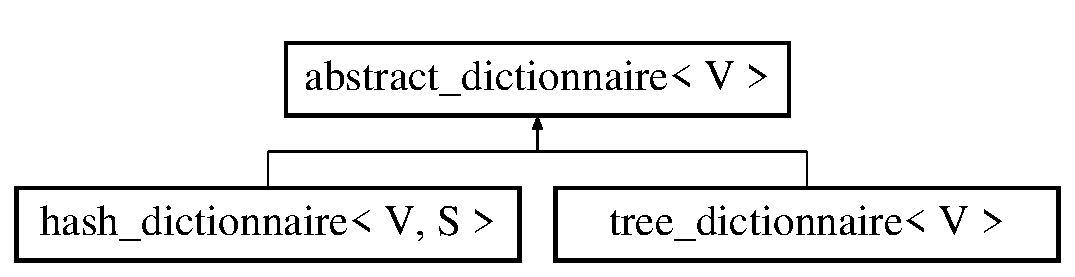
\includegraphics[height=2.000000cm]{classabstract__dictionnaire}
\end{center}
\end{figure}
\subsection*{Fonctions membres publiques}
\begin{DoxyCompactItemize}
\item 
\hypertarget{classabstract__dictionnaire_a222d289fc3bdd6c0e4911509e7fa855d}{virtual \hyperlink{classabstract__dictionnaire_a222d289fc3bdd6c0e4911509e7fa855d}{$\sim$abstract\-\_\-dictionnaire} ()}\label{classabstract__dictionnaire_a222d289fc3bdd6c0e4911509e7fa855d}

\begin{DoxyCompactList}\small\item\em Destructeur virtuel. \end{DoxyCompactList}\item 
virtual ostream \& \hyperlink{classabstract__dictionnaire_ae472681c840b81cfc512b47dc664774c}{afficher} (ostream \&os=cout) const =0
\begin{DoxyCompactList}\small\item\em Affiche le dictionnaire sur le flux passé en paramètre. \end{DoxyCompactList}\item 
virtual bool \hyperlink{classabstract__dictionnaire_abeb4f33d1600bcf2a6058f7bdae65aaf}{contient\-Mot} (const string \&mot) const =0
\begin{DoxyCompactList}\small\item\em Teste si le dictionnaire contient un mot. \end{DoxyCompactList}\item 
virtual void \hyperlink{classabstract__dictionnaire_a0c3af73e050ee04b8a14161052c5e636}{ajouter\-Mot} (const string \&mot, const V \&v)=0
\begin{DoxyCompactList}\small\item\em Ajoute la chaîne mot au dictionnaire, avec la valeur v, mot étant supposé absent du dictionnaire. \end{DoxyCompactList}\item 
virtual void \hyperlink{classabstract__dictionnaire_a3d19bb8707514928a5f54e73701f0d1c}{associer\-Mot} (const string \&mot, const V \&v)=0
\begin{DoxyCompactList}\small\item\em Associe la valeur v à la chaîne mot dans le dictionnaire, mot pouvant être présent ou absent du dictionnaire. \end{DoxyCompactList}\item 
virtual void \hyperlink{classabstract__dictionnaire_a7063c0c484fe9eabecb0ddb268951823}{supprimer\-Mot} (const string \&mot)=0
\begin{DoxyCompactList}\small\item\em Supprime l'éventuelle chaîne mot du dictionnaire. \end{DoxyCompactList}\item 
virtual V \hyperlink{classabstract__dictionnaire_abf2426d66e5499582dc4dc4fe5eeb1c3}{valeur\-Associee} (const string \&mot) const =0
\begin{DoxyCompactList}\small\item\em Donne la valeur correspondant à la chaîne mot (supposée figurer dans le dictionnaire). \end{DoxyCompactList}\item 
virtual \hyperlink{structtriplet}{triplet}$<$ string $\ast$, V \\*
$\ast$, int $>$ \hyperlink{classabstract__dictionnaire_a0b04fb9d2062846f5c9bdc8c7742538f}{to\-\_\-array} () const =0
\begin{DoxyCompactList}\small\item\em Retourne un triplet contenant le tableau des mots du dictionnaire, le tableau des valeurs associées aux mots et la taille de ces tableaux. \end{DoxyCompactList}\item 
virtual void \hyperlink{classabstract__dictionnaire_a0bebd25d66714c37c11f53f0797b2ffd}{to\-\_\-list} (list$<$ pair$<$ string, V $>$ $>$ \&ls) const =0
\begin{DoxyCompactList}\small\item\em Charge les mots et les valeurs du dictionnaire dans la liste passée en paramètre. \end{DoxyCompactList}\end{DoxyCompactItemize}


\subsection{Description détaillée}
\subsubsection*{template$<$typename V$>$class abstract\-\_\-dictionnaire$<$ V $>$}

Classe abstraite \hyperlink{classabstract__dictionnaire}{abstract\-\_\-dictionnaire}. 

\subsection{Documentation des fonctions membres}
\hypertarget{classabstract__dictionnaire_ae472681c840b81cfc512b47dc664774c}{\index{abstract\-\_\-dictionnaire@{abstract\-\_\-dictionnaire}!afficher@{afficher}}
\index{afficher@{afficher}!abstract_dictionnaire@{abstract\-\_\-dictionnaire}}
\subsubsection[{afficher}]{\setlength{\rightskip}{0pt plus 5cm}template$<$typename V$>$ virtual ostream\& {\bf abstract\-\_\-dictionnaire}$<$ V $>$\-::afficher (
\begin{DoxyParamCaption}
\item[{ostream \&}]{os = {\ttfamily cout}}
\end{DoxyParamCaption}
) const\hspace{0.3cm}{\ttfamily [pure virtual]}}}\label{classabstract__dictionnaire_ae472681c840b81cfc512b47dc664774c}


Affiche le dictionnaire sur le flux passé en paramètre. 


\begin{DoxyParams}{Paramètres}
{\em os} & \-: le flux de sortie \\
\hline
\end{DoxyParams}
\begin{DoxyReturn}{Renvoie}
le flux de sortie 
\end{DoxyReturn}


Implémenté dans \hyperlink{classhash__dictionnaire_a900870781ea0d8b4d6821bef1046495a}{hash\-\_\-dictionnaire$<$ V, S $>$}, et \hyperlink{classtree__dictionnaire_af8386fa4ca1a5d86ca73d2e1f7845999}{tree\-\_\-dictionnaire$<$ V $>$}.

\hypertarget{classabstract__dictionnaire_a0c3af73e050ee04b8a14161052c5e636}{\index{abstract\-\_\-dictionnaire@{abstract\-\_\-dictionnaire}!ajouter\-Mot@{ajouter\-Mot}}
\index{ajouter\-Mot@{ajouter\-Mot}!abstract_dictionnaire@{abstract\-\_\-dictionnaire}}
\subsubsection[{ajouter\-Mot}]{\setlength{\rightskip}{0pt plus 5cm}template$<$typename V$>$ virtual void {\bf abstract\-\_\-dictionnaire}$<$ V $>$\-::ajouter\-Mot (
\begin{DoxyParamCaption}
\item[{const string \&}]{mot, }
\item[{const V \&}]{v}
\end{DoxyParamCaption}
)\hspace{0.3cm}{\ttfamily [pure virtual]}}}\label{classabstract__dictionnaire_a0c3af73e050ee04b8a14161052c5e636}


Ajoute la chaîne mot au dictionnaire, avec la valeur v, mot étant supposé absent du dictionnaire. 


\begin{DoxyParams}{Paramètres}
{\em mot} & \-: le mot à ajouter \\
\hline
{\em v} & \-: la valeur associée au mot \\
\hline
\end{DoxyParams}


Implémenté dans \hyperlink{classhash__dictionnaire_a7686074b9b747fd3be2423d0faffa546}{hash\-\_\-dictionnaire$<$ V, S $>$}, et \hyperlink{classtree__dictionnaire_a867e2a62ee1defe00f00c08e170192d1}{tree\-\_\-dictionnaire$<$ V $>$}.

\hypertarget{classabstract__dictionnaire_a3d19bb8707514928a5f54e73701f0d1c}{\index{abstract\-\_\-dictionnaire@{abstract\-\_\-dictionnaire}!associer\-Mot@{associer\-Mot}}
\index{associer\-Mot@{associer\-Mot}!abstract_dictionnaire@{abstract\-\_\-dictionnaire}}
\subsubsection[{associer\-Mot}]{\setlength{\rightskip}{0pt plus 5cm}template$<$typename V$>$ virtual void {\bf abstract\-\_\-dictionnaire}$<$ V $>$\-::associer\-Mot (
\begin{DoxyParamCaption}
\item[{const string \&}]{mot, }
\item[{const V \&}]{v}
\end{DoxyParamCaption}
)\hspace{0.3cm}{\ttfamily [pure virtual]}}}\label{classabstract__dictionnaire_a3d19bb8707514928a5f54e73701f0d1c}


Associe la valeur v à la chaîne mot dans le dictionnaire, mot pouvant être présent ou absent du dictionnaire. 


\begin{DoxyParams}{Paramètres}
{\em mot} & \-: le mot à modifier \\
\hline
{\em v} & \-: la valeur associée au mot \\
\hline
\end{DoxyParams}


Implémenté dans \hyperlink{classhash__dictionnaire_aa018c9fc0e0a343cf2c30ba4d9a5fc1e}{hash\-\_\-dictionnaire$<$ V, S $>$}, et \hyperlink{classtree__dictionnaire_afc52a48eea27916d31c7088813e83fd0}{tree\-\_\-dictionnaire$<$ V $>$}.

\hypertarget{classabstract__dictionnaire_abeb4f33d1600bcf2a6058f7bdae65aaf}{\index{abstract\-\_\-dictionnaire@{abstract\-\_\-dictionnaire}!contient\-Mot@{contient\-Mot}}
\index{contient\-Mot@{contient\-Mot}!abstract_dictionnaire@{abstract\-\_\-dictionnaire}}
\subsubsection[{contient\-Mot}]{\setlength{\rightskip}{0pt plus 5cm}template$<$typename V$>$ virtual bool {\bf abstract\-\_\-dictionnaire}$<$ V $>$\-::contient\-Mot (
\begin{DoxyParamCaption}
\item[{const string \&}]{mot}
\end{DoxyParamCaption}
) const\hspace{0.3cm}{\ttfamily [pure virtual]}}}\label{classabstract__dictionnaire_abeb4f33d1600bcf2a6058f7bdae65aaf}


Teste si le dictionnaire contient un mot. 


\begin{DoxyParams}{Paramètres}
{\em mot} & \-: le mot recherché \\
\hline
\end{DoxyParams}
\begin{DoxyReturn}{Renvoie}
vrai si le dictionnaire contient le mot sinon faux 
\end{DoxyReturn}


Implémenté dans \hyperlink{classhash__dictionnaire_a4e39ddc24269bbec246bdf0180670643}{hash\-\_\-dictionnaire$<$ V, S $>$}, et \hyperlink{classtree__dictionnaire_a688203a2da7bbc1bdb667868ef6e18a3}{tree\-\_\-dictionnaire$<$ V $>$}.

\hypertarget{classabstract__dictionnaire_a7063c0c484fe9eabecb0ddb268951823}{\index{abstract\-\_\-dictionnaire@{abstract\-\_\-dictionnaire}!supprimer\-Mot@{supprimer\-Mot}}
\index{supprimer\-Mot@{supprimer\-Mot}!abstract_dictionnaire@{abstract\-\_\-dictionnaire}}
\subsubsection[{supprimer\-Mot}]{\setlength{\rightskip}{0pt plus 5cm}template$<$typename V$>$ virtual void {\bf abstract\-\_\-dictionnaire}$<$ V $>$\-::supprimer\-Mot (
\begin{DoxyParamCaption}
\item[{const string \&}]{mot}
\end{DoxyParamCaption}
)\hspace{0.3cm}{\ttfamily [pure virtual]}}}\label{classabstract__dictionnaire_a7063c0c484fe9eabecb0ddb268951823}


Supprime l'éventuelle chaîne mot du dictionnaire. 


\begin{DoxyParams}{Paramètres}
{\em mot} & \-: le mot à supprimer \\
\hline
\end{DoxyParams}


Implémenté dans \hyperlink{classhash__dictionnaire_a65edff55e6785b5d6d6db97293330368}{hash\-\_\-dictionnaire$<$ V, S $>$}, et \hyperlink{classtree__dictionnaire_a76fa52ac010b861d437b87d1b68fe0cc}{tree\-\_\-dictionnaire$<$ V $>$}.

\hypertarget{classabstract__dictionnaire_a0b04fb9d2062846f5c9bdc8c7742538f}{\index{abstract\-\_\-dictionnaire@{abstract\-\_\-dictionnaire}!to\-\_\-array@{to\-\_\-array}}
\index{to\-\_\-array@{to\-\_\-array}!abstract_dictionnaire@{abstract\-\_\-dictionnaire}}
\subsubsection[{to\-\_\-array}]{\setlength{\rightskip}{0pt plus 5cm}template$<$typename V$>$ virtual {\bf triplet}$<$string$\ast$,V$\ast$,int$>$ {\bf abstract\-\_\-dictionnaire}$<$ V $>$\-::to\-\_\-array (
\begin{DoxyParamCaption}
{}
\end{DoxyParamCaption}
) const\hspace{0.3cm}{\ttfamily [pure virtual]}}}\label{classabstract__dictionnaire_a0b04fb9d2062846f5c9bdc8c7742538f}


Retourne un triplet contenant le tableau des mots du dictionnaire, le tableau des valeurs associées aux mots et la taille de ces tableaux. 

\begin{DoxyRefDesc}{Obsolète}
\item[\hyperlink{deprecated__deprecated000001}{Obsolète}]utiliser \hyperlink{classabstract__dictionnaire_a0bebd25d66714c37c11f53f0797b2ffd}{to\-\_\-list()} \end{DoxyRefDesc}
\begin{DoxyReturn}{Renvoie}
le triplet mots-\/valeurs-\/taille 
\end{DoxyReturn}


Implémenté dans \hyperlink{classhash__dictionnaire_a4ea9ee40aa51412199f64a6dce55842d}{hash\-\_\-dictionnaire$<$ V, S $>$}, et \hyperlink{classtree__dictionnaire_a1a5c6cd5954ceac7adbd09eb390f610c}{tree\-\_\-dictionnaire$<$ V $>$}.

\hypertarget{classabstract__dictionnaire_a0bebd25d66714c37c11f53f0797b2ffd}{\index{abstract\-\_\-dictionnaire@{abstract\-\_\-dictionnaire}!to\-\_\-list@{to\-\_\-list}}
\index{to\-\_\-list@{to\-\_\-list}!abstract_dictionnaire@{abstract\-\_\-dictionnaire}}
\subsubsection[{to\-\_\-list}]{\setlength{\rightskip}{0pt plus 5cm}template$<$typename V$>$ virtual void {\bf abstract\-\_\-dictionnaire}$<$ V $>$\-::to\-\_\-list (
\begin{DoxyParamCaption}
\item[{list$<$ pair$<$ string, V $>$ $>$ \&}]{ls}
\end{DoxyParamCaption}
) const\hspace{0.3cm}{\ttfamily [pure virtual]}}}\label{classabstract__dictionnaire_a0bebd25d66714c37c11f53f0797b2ffd}


Charge les mots et les valeurs du dictionnaire dans la liste passée en paramètre. 


\begin{DoxyParams}{Paramètres}
{\em ls} & \-: la liste où charger les couples mot-\/valeur \\
\hline
\end{DoxyParams}


Implémenté dans \hyperlink{classhash__dictionnaire_ac307646722314ba8898c544f485eae8a}{hash\-\_\-dictionnaire$<$ V, S $>$}, et \hyperlink{classtree__dictionnaire_a5e251a8b18b85bf416729ddde96242b6}{tree\-\_\-dictionnaire$<$ V $>$}.

\hypertarget{classabstract__dictionnaire_abf2426d66e5499582dc4dc4fe5eeb1c3}{\index{abstract\-\_\-dictionnaire@{abstract\-\_\-dictionnaire}!valeur\-Associee@{valeur\-Associee}}
\index{valeur\-Associee@{valeur\-Associee}!abstract_dictionnaire@{abstract\-\_\-dictionnaire}}
\subsubsection[{valeur\-Associee}]{\setlength{\rightskip}{0pt plus 5cm}template$<$typename V$>$ virtual V {\bf abstract\-\_\-dictionnaire}$<$ V $>$\-::valeur\-Associee (
\begin{DoxyParamCaption}
\item[{const string \&}]{mot}
\end{DoxyParamCaption}
) const\hspace{0.3cm}{\ttfamily [pure virtual]}}}\label{classabstract__dictionnaire_abf2426d66e5499582dc4dc4fe5eeb1c3}


Donne la valeur correspondant à la chaîne mot (supposée figurer dans le dictionnaire). 


\begin{DoxyParams}{Paramètres}
{\em mot} & \-: le mot dont on veut récupérer la valeur associée \\
\hline
\end{DoxyParams}
\begin{DoxyReturn}{Renvoie}
la valeur associée au mot 
\end{DoxyReturn}


Implémenté dans \hyperlink{classhash__dictionnaire_a7b7b3c0023fa68a6932d839feda7c1f2}{hash\-\_\-dictionnaire$<$ V, S $>$}, et \hyperlink{classtree__dictionnaire_a7fb5e78b2bf0d5e75c9aebb870d43879}{tree\-\_\-dictionnaire$<$ V $>$}.



La documentation de cette classe a été générée à partir du fichier suivant \-:\begin{DoxyCompactItemize}
\item 
/home/grdx/git/cpp-\/collections/src/\hyperlink{abstract__dictionnaire_8hpp}{abstract\-\_\-dictionnaire.\-hpp}\end{DoxyCompactItemize}

\hypertarget{classhash__dictionnaire}{\section{Référence du modèle de la classe hash\-\_\-dictionnaire$<$ V, S $>$}
\label{classhash__dictionnaire}\index{hash\-\_\-dictionnaire$<$ V, S $>$@{hash\-\_\-dictionnaire$<$ V, S $>$}}
}


Classe \hyperlink{classhash__dictionnaire}{hash\-\_\-dictionnaire} implémente la classe abstraite \hyperlink{classabstract__dictionnaire}{abstract\-\_\-dictionnaire} avec une table de hachage. V le type des valeurs associées aux mots.  




{\ttfamily \#include $<$hash\-\_\-dictionnaire.\-hpp$>$}

Graphe d'héritage de hash\-\_\-dictionnaire$<$ V, S $>$\-:\begin{figure}[H]
\begin{center}
\leavevmode
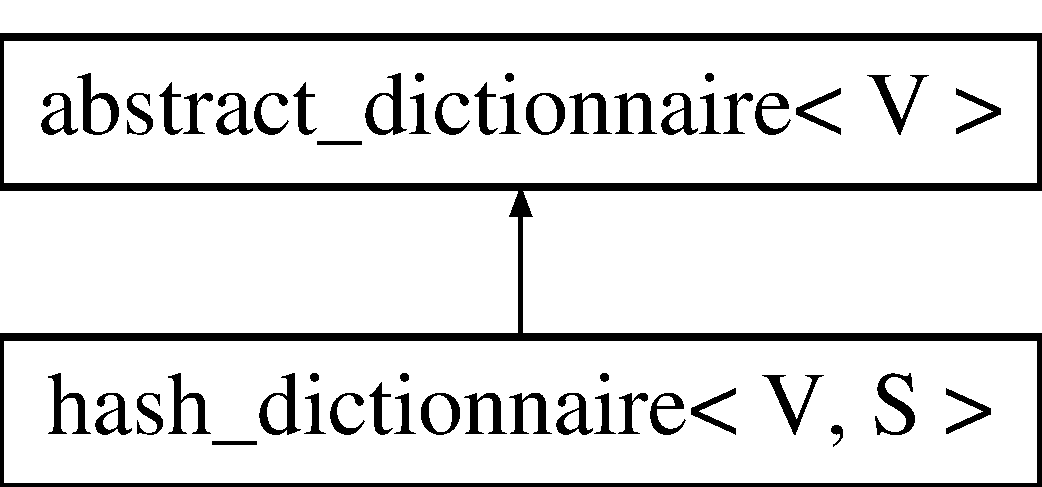
\includegraphics[height=2.000000cm]{classhash__dictionnaire}
\end{center}
\end{figure}
\subsection*{Fonctions membres publiques}
\begin{DoxyCompactItemize}
\item 
\hypertarget{classhash__dictionnaire_a381e1d57c7bd7d74aaf16ca6c44056d7}{\hyperlink{classhash__dictionnaire_a381e1d57c7bd7d74aaf16ca6c44056d7}{hash\-\_\-dictionnaire} ()}\label{classhash__dictionnaire_a381e1d57c7bd7d74aaf16ca6c44056d7}

\begin{DoxyCompactList}\small\item\em Constructeur. O(1) \end{DoxyCompactList}\item 
\hypertarget{classhash__dictionnaire_a17ea93b8a231a3f54d49197c5cfca700}{\hyperlink{classhash__dictionnaire_a17ea93b8a231a3f54d49197c5cfca700}{$\sim$hash\-\_\-dictionnaire} ()}\label{classhash__dictionnaire_a17ea93b8a231a3f54d49197c5cfca700}

\begin{DoxyCompactList}\small\item\em Destructeur. O(n) \end{DoxyCompactList}\item 
ostream \& \hyperlink{classhash__dictionnaire_a900870781ea0d8b4d6821bef1046495a}{afficher} (ostream \&os=cout) const 
\begin{DoxyCompactList}\small\item\em Affiche le dictionnaire sur le flux passé en paramètre. O(n) \end{DoxyCompactList}\item 
bool \hyperlink{classhash__dictionnaire_a4e39ddc24269bbec246bdf0180670643}{contient\-Mot} (const string \&mot) const 
\begin{DoxyCompactList}\small\item\em Teste si le dictionnaire contient un mot. O(n) \end{DoxyCompactList}\item 
void \hyperlink{classhash__dictionnaire_a7686074b9b747fd3be2423d0faffa546}{ajouter\-Mot} (const string \&mot, const V \&v)
\begin{DoxyCompactList}\small\item\em Ajoute la chaîne mot au dictionnaire, avec la valeur v, mot étant supposé absent du dictionnaire. O(n) \end{DoxyCompactList}\item 
void \hyperlink{classhash__dictionnaire_aa018c9fc0e0a343cf2c30ba4d9a5fc1e}{associer\-Mot} (const string \&mot, const V \&v)
\begin{DoxyCompactList}\small\item\em Associe la valeur v à la chaîne mot dans le dictionnaire, mot pouvant être présent ou absent du dictionnaire. O(n) \end{DoxyCompactList}\item 
void \hyperlink{classhash__dictionnaire_a65edff55e6785b5d6d6db97293330368}{supprimer\-Mot} (const string \&mot)
\begin{DoxyCompactList}\small\item\em Supprime l'éventuelle chaîne mot du dictionnaire. O(n) \end{DoxyCompactList}\item 
V \hyperlink{classhash__dictionnaire_a7b7b3c0023fa68a6932d839feda7c1f2}{valeur\-Associee} (const string \&mot) const 
\begin{DoxyCompactList}\small\item\em Donne la valeur correspondant à la chaîne mot (supposée figurer dans le dictionnaire). O(n) \end{DoxyCompactList}\item 
\hyperlink{structtriplet}{triplet}$<$ string $\ast$, V $\ast$, int $>$ \hyperlink{classhash__dictionnaire_a4ea9ee40aa51412199f64a6dce55842d}{to\-\_\-array} () const 
\begin{DoxyCompactList}\small\item\em Retourne un triplet contenant le tableau des mots du dictionnaire, le tableau des valeurs associées aux mots et la taille de ces tableaux. O(n) \end{DoxyCompactList}\item 
void \hyperlink{classhash__dictionnaire_ac307646722314ba8898c544f485eae8a}{to\-\_\-list} (list$<$ pair$<$ string, V $>$ $>$ \&ls) const 
\begin{DoxyCompactList}\small\item\em Charge les mots et les valeurs du dictionnaire dans la liste passée en paramètre. O(n) \end{DoxyCompactList}\end{DoxyCompactItemize}
\subsection*{Attributs protégés}
\begin{DoxyCompactItemize}
\item 
\hypertarget{classhash__dictionnaire_a32ee1b9b8aa689c4ae7d54af4d8c3140}{\hyperlink{classhash__table}{hash\-\_\-table}$<$ string, V, S $>$ {\bfseries \-\_\-data}}\label{classhash__dictionnaire_a32ee1b9b8aa689c4ae7d54af4d8c3140}

\end{DoxyCompactItemize}


\subsection{Description détaillée}
\subsubsection*{template$<$typename V, int S = 26$>$class hash\-\_\-dictionnaire$<$ V, S $>$}

Classe \hyperlink{classhash__dictionnaire}{hash\-\_\-dictionnaire} implémente la classe abstraite \hyperlink{classabstract__dictionnaire}{abstract\-\_\-dictionnaire} avec une table de hachage. V le type des valeurs associées aux mots. 

\subsection{Documentation des fonctions membres}
\hypertarget{classhash__dictionnaire_a900870781ea0d8b4d6821bef1046495a}{\index{hash\-\_\-dictionnaire@{hash\-\_\-dictionnaire}!afficher@{afficher}}
\index{afficher@{afficher}!hash_dictionnaire@{hash\-\_\-dictionnaire}}
\subsubsection[{afficher}]{\setlength{\rightskip}{0pt plus 5cm}template$<$typename V , int S$>$ ostream \& {\bf hash\-\_\-dictionnaire}$<$ V, S $>$\-::afficher (
\begin{DoxyParamCaption}
\item[{ostream \&}]{os = {\ttfamily cout}}
\end{DoxyParamCaption}
) const\hspace{0.3cm}{\ttfamily [virtual]}}}\label{classhash__dictionnaire_a900870781ea0d8b4d6821bef1046495a}


Affiche le dictionnaire sur le flux passé en paramètre. O(n) 


\begin{DoxyParams}{Paramètres}
{\em os} & \-: le flux de sortie \\
\hline
\end{DoxyParams}
\begin{DoxyReturn}{Renvoie}
le flux de sortie 
\end{DoxyReturn}


Implémente \hyperlink{classabstract__dictionnaire_ae472681c840b81cfc512b47dc664774c}{abstract\-\_\-dictionnaire$<$ V $>$}.

\hypertarget{classhash__dictionnaire_a7686074b9b747fd3be2423d0faffa546}{\index{hash\-\_\-dictionnaire@{hash\-\_\-dictionnaire}!ajouter\-Mot@{ajouter\-Mot}}
\index{ajouter\-Mot@{ajouter\-Mot}!hash_dictionnaire@{hash\-\_\-dictionnaire}}
\subsubsection[{ajouter\-Mot}]{\setlength{\rightskip}{0pt plus 5cm}template$<$typename V , int S$>$ void {\bf hash\-\_\-dictionnaire}$<$ V, S $>$\-::ajouter\-Mot (
\begin{DoxyParamCaption}
\item[{const string \&}]{mot, }
\item[{const V \&}]{v}
\end{DoxyParamCaption}
)\hspace{0.3cm}{\ttfamily [virtual]}}}\label{classhash__dictionnaire_a7686074b9b747fd3be2423d0faffa546}


Ajoute la chaîne mot au dictionnaire, avec la valeur v, mot étant supposé absent du dictionnaire. O(n) 


\begin{DoxyParams}{Paramètres}
{\em mot} & \-: le mot à ajouter \\
\hline
{\em v} & \-: la valeur associée au mot \\
\hline
\end{DoxyParams}


Implémente \hyperlink{classabstract__dictionnaire_a0c3af73e050ee04b8a14161052c5e636}{abstract\-\_\-dictionnaire$<$ V $>$}.

\hypertarget{classhash__dictionnaire_aa018c9fc0e0a343cf2c30ba4d9a5fc1e}{\index{hash\-\_\-dictionnaire@{hash\-\_\-dictionnaire}!associer\-Mot@{associer\-Mot}}
\index{associer\-Mot@{associer\-Mot}!hash_dictionnaire@{hash\-\_\-dictionnaire}}
\subsubsection[{associer\-Mot}]{\setlength{\rightskip}{0pt plus 5cm}template$<$typename V , int S$>$ void {\bf hash\-\_\-dictionnaire}$<$ V, S $>$\-::associer\-Mot (
\begin{DoxyParamCaption}
\item[{const string \&}]{mot, }
\item[{const V \&}]{v}
\end{DoxyParamCaption}
)\hspace{0.3cm}{\ttfamily [virtual]}}}\label{classhash__dictionnaire_aa018c9fc0e0a343cf2c30ba4d9a5fc1e}


Associe la valeur v à la chaîne mot dans le dictionnaire, mot pouvant être présent ou absent du dictionnaire. O(n) 


\begin{DoxyParams}{Paramètres}
{\em mot} & \-: le mot à modifier \\
\hline
{\em v} & \-: la valeur associée au mot \\
\hline
\end{DoxyParams}


Implémente \hyperlink{classabstract__dictionnaire_a3d19bb8707514928a5f54e73701f0d1c}{abstract\-\_\-dictionnaire$<$ V $>$}.

\hypertarget{classhash__dictionnaire_a4e39ddc24269bbec246bdf0180670643}{\index{hash\-\_\-dictionnaire@{hash\-\_\-dictionnaire}!contient\-Mot@{contient\-Mot}}
\index{contient\-Mot@{contient\-Mot}!hash_dictionnaire@{hash\-\_\-dictionnaire}}
\subsubsection[{contient\-Mot}]{\setlength{\rightskip}{0pt plus 5cm}template$<$typename V , int S$>$ bool {\bf hash\-\_\-dictionnaire}$<$ V, S $>$\-::contient\-Mot (
\begin{DoxyParamCaption}
\item[{const string \&}]{mot}
\end{DoxyParamCaption}
) const\hspace{0.3cm}{\ttfamily [virtual]}}}\label{classhash__dictionnaire_a4e39ddc24269bbec246bdf0180670643}


Teste si le dictionnaire contient un mot. O(n) 


\begin{DoxyParams}{Paramètres}
{\em mot} & \-: le mot recherché \\
\hline
\end{DoxyParams}
\begin{DoxyReturn}{Renvoie}
vrai si le dictionnaire contient le mot sinon faux 
\end{DoxyReturn}


Implémente \hyperlink{classabstract__dictionnaire_abeb4f33d1600bcf2a6058f7bdae65aaf}{abstract\-\_\-dictionnaire$<$ V $>$}.

\hypertarget{classhash__dictionnaire_a65edff55e6785b5d6d6db97293330368}{\index{hash\-\_\-dictionnaire@{hash\-\_\-dictionnaire}!supprimer\-Mot@{supprimer\-Mot}}
\index{supprimer\-Mot@{supprimer\-Mot}!hash_dictionnaire@{hash\-\_\-dictionnaire}}
\subsubsection[{supprimer\-Mot}]{\setlength{\rightskip}{0pt plus 5cm}template$<$typename V , int S$>$ void {\bf hash\-\_\-dictionnaire}$<$ V, S $>$\-::supprimer\-Mot (
\begin{DoxyParamCaption}
\item[{const string \&}]{mot}
\end{DoxyParamCaption}
)\hspace{0.3cm}{\ttfamily [virtual]}}}\label{classhash__dictionnaire_a65edff55e6785b5d6d6db97293330368}


Supprime l'éventuelle chaîne mot du dictionnaire. O(n) 


\begin{DoxyParams}{Paramètres}
{\em mot} & \-: le mot à supprimer \\
\hline
\end{DoxyParams}


Implémente \hyperlink{classabstract__dictionnaire_a7063c0c484fe9eabecb0ddb268951823}{abstract\-\_\-dictionnaire$<$ V $>$}.

\hypertarget{classhash__dictionnaire_a4ea9ee40aa51412199f64a6dce55842d}{\index{hash\-\_\-dictionnaire@{hash\-\_\-dictionnaire}!to\-\_\-array@{to\-\_\-array}}
\index{to\-\_\-array@{to\-\_\-array}!hash_dictionnaire@{hash\-\_\-dictionnaire}}
\subsubsection[{to\-\_\-array}]{\setlength{\rightskip}{0pt plus 5cm}template$<$typename V , int S$>$ {\bf triplet}$<$ string $\ast$, V $\ast$, int $>$ {\bf hash\-\_\-dictionnaire}$<$ V, S $>$\-::to\-\_\-array (
\begin{DoxyParamCaption}
{}
\end{DoxyParamCaption}
) const\hspace{0.3cm}{\ttfamily [virtual]}}}\label{classhash__dictionnaire_a4ea9ee40aa51412199f64a6dce55842d}


Retourne un triplet contenant le tableau des mots du dictionnaire, le tableau des valeurs associées aux mots et la taille de ces tableaux. O(n) 

\begin{DoxyRefDesc}{Obsolète}
\item[\hyperlink{deprecated__deprecated000002}{Obsolète}]utiliser \hyperlink{classhash__dictionnaire_ac307646722314ba8898c544f485eae8a}{to\-\_\-list()} \end{DoxyRefDesc}
\begin{DoxyReturn}{Renvoie}
le triplet mots-\/valeurs-\/taille 
\end{DoxyReturn}


Implémente \hyperlink{classabstract__dictionnaire_a0b04fb9d2062846f5c9bdc8c7742538f}{abstract\-\_\-dictionnaire$<$ V $>$}.

\hypertarget{classhash__dictionnaire_ac307646722314ba8898c544f485eae8a}{\index{hash\-\_\-dictionnaire@{hash\-\_\-dictionnaire}!to\-\_\-list@{to\-\_\-list}}
\index{to\-\_\-list@{to\-\_\-list}!hash_dictionnaire@{hash\-\_\-dictionnaire}}
\subsubsection[{to\-\_\-list}]{\setlength{\rightskip}{0pt plus 5cm}template$<$typename V , int S$>$ void {\bf hash\-\_\-dictionnaire}$<$ V, S $>$\-::to\-\_\-list (
\begin{DoxyParamCaption}
\item[{list$<$ pair$<$ string, V $>$ $>$ \&}]{ls}
\end{DoxyParamCaption}
) const\hspace{0.3cm}{\ttfamily [virtual]}}}\label{classhash__dictionnaire_ac307646722314ba8898c544f485eae8a}


Charge les mots et les valeurs du dictionnaire dans la liste passée en paramètre. O(n) 


\begin{DoxyParams}{Paramètres}
{\em ls} & \-: la liste où charger les couples mot-\/valeur \\
\hline
\end{DoxyParams}


Implémente \hyperlink{classabstract__dictionnaire_a0bebd25d66714c37c11f53f0797b2ffd}{abstract\-\_\-dictionnaire$<$ V $>$}.

\hypertarget{classhash__dictionnaire_a7b7b3c0023fa68a6932d839feda7c1f2}{\index{hash\-\_\-dictionnaire@{hash\-\_\-dictionnaire}!valeur\-Associee@{valeur\-Associee}}
\index{valeur\-Associee@{valeur\-Associee}!hash_dictionnaire@{hash\-\_\-dictionnaire}}
\subsubsection[{valeur\-Associee}]{\setlength{\rightskip}{0pt plus 5cm}template$<$typename V , int S$>$ V {\bf hash\-\_\-dictionnaire}$<$ V, S $>$\-::valeur\-Associee (
\begin{DoxyParamCaption}
\item[{const string \&}]{mot}
\end{DoxyParamCaption}
) const\hspace{0.3cm}{\ttfamily [virtual]}}}\label{classhash__dictionnaire_a7b7b3c0023fa68a6932d839feda7c1f2}


Donne la valeur correspondant à la chaîne mot (supposée figurer dans le dictionnaire). O(n) 


\begin{DoxyParams}{Paramètres}
{\em mot} & \-: le mot dont on veut récupérer la valeur associée \\
\hline
\end{DoxyParams}
\begin{DoxyReturn}{Renvoie}
la valeur associée au mot 
\end{DoxyReturn}


Implémente \hyperlink{classabstract__dictionnaire_abf2426d66e5499582dc4dc4fe5eeb1c3}{abstract\-\_\-dictionnaire$<$ V $>$}.



La documentation de cette classe a été générée à partir du fichier suivant \-:\begin{DoxyCompactItemize}
\item 
/home/grdx/git/cpp-\/collections/src/\hyperlink{hash__dictionnaire_8hpp}{hash\-\_\-dictionnaire.\-hpp}\end{DoxyCompactItemize}

\hypertarget{classhash__table}{\section{Référence du modèle de la classe hash\-\_\-table$<$ K, V, S $>$}
\label{classhash__table}\index{hash\-\_\-table$<$ K, V, S $>$@{hash\-\_\-table$<$ K, V, S $>$}}
}


Implémentation générique d'une table de hachage avec taleaux associatifs. K le type des clefs, V le type des valeurs et S le nombre de maps.  




{\ttfamily \#include $<$hash\-\_\-table.\-hpp$>$}

\subsection*{Fonctions membres publiques}
\begin{DoxyCompactItemize}
\item 
\hypertarget{classhash__table_ae070d734af1d6d8cf2ba85ab68f363b8}{\hyperlink{classhash__table_ae070d734af1d6d8cf2ba85ab68f363b8}{hash\-\_\-table} ()}\label{classhash__table_ae070d734af1d6d8cf2ba85ab68f363b8}

\begin{DoxyCompactList}\small\item\em Constructeur. O(1) \end{DoxyCompactList}\item 
\hypertarget{classhash__table_a745737dbcbb3da989e94d587aa94cf2f}{\hyperlink{classhash__table_a745737dbcbb3da989e94d587aa94cf2f}{$\sim$hash\-\_\-table} ()}\label{classhash__table_a745737dbcbb3da989e94d587aa94cf2f}

\begin{DoxyCompactList}\small\item\em Destructeur. O(n) \end{DoxyCompactList}\item 
\hypertarget{classhash__table_a842112e2fa64ea1b80f5983e2308e6db}{void \hyperlink{classhash__table_a842112e2fa64ea1b80f5983e2308e6db}{clear} ()}\label{classhash__table_a842112e2fa64ea1b80f5983e2308e6db}

\begin{DoxyCompactList}\small\item\em Vide la \hyperlink{classhash__table}{hash\-\_\-table}. O(n) \end{DoxyCompactList}\item 
bool \hyperlink{classhash__table_a95b8f8d9a6704841ec1c84dda4959329}{contains\-\_\-key} (const K \&key) const 
\begin{DoxyCompactList}\small\item\em Retourne vrai si la \hyperlink{classhash__table}{hash\-\_\-table} contient la clef key, retourne faux dans le cas contraire. O(n) \end{DoxyCompactList}\item 
bool \hyperlink{classhash__table_a317e71765a840583fe81afa8f7a431ca}{contains\-\_\-value} (const V \&value) const 
\begin{DoxyCompactList}\small\item\em Retourne vrai si la \hyperlink{classhash__table}{hash\-\_\-table} contient la valeur value, retourne faux dans le cas contraire. O(n) \end{DoxyCompactList}\item 
V \hyperlink{classhash__table_a91816c9092bd1b98ca52a0955df43752}{get} (const K \&key) const 
\begin{DoxyCompactList}\small\item\em Retourne la valeur associée à la clef key si la \hyperlink{classhash__table}{hash\-\_\-table} contient la clef key, lève une exception dans le cas contraire. O(n) \end{DoxyCompactList}\item 
V \& \hyperlink{classhash__table_a3a8ce67c4dd3952ca1a5b05f2ed0b5a6}{get\-\_\-ref} (const K \&key) const 
\begin{DoxyCompactList}\small\item\em Retourne la référence de la valeur associée à la clef key si la \hyperlink{classhash__table}{hash\-\_\-table} contient la clef key, lève une exception dans le cas contraire. O(n) \end{DoxyCompactList}\item 
bool \hyperlink{classhash__table_a3a81ed200333cf7fd4745ed6f0195fd3}{is\-\_\-empty} () const 
\begin{DoxyCompactList}\small\item\em Retourne vrai si la \hyperlink{classhash__table}{hash\-\_\-table} est vide, retourne faux dans le cas contraire. O(1) \end{DoxyCompactList}\item 
K $\ast$ \hyperlink{classhash__table_aa65cffb759b4b5f480e71bf59f8268db}{keys\-\_\-array} () const 
\begin{DoxyCompactList}\small\item\em Retourne un tableau contenant toutes les clefs de la \hyperlink{classhash__table}{hash\-\_\-table}. O(n) \end{DoxyCompactList}\item 
bool \hyperlink{classhash__table_a91998dee99f2f09b0cff2ff578724edf}{put} (const K \&key, const V \&value)
\begin{DoxyCompactList}\small\item\em Ajoute un nouveau couple clef-\/valeur à la \hyperlink{classhash__table}{hash\-\_\-table} si celle-\/ci ne contient pas la clef key, si la \hyperlink{classhash__table}{hash\-\_\-table} contient la clef key alors la valeur associée à la clef sera remplacée par value. O(n) \end{DoxyCompactList}\item 
bool \hyperlink{classhash__table_a7d5896c24c5bf2518fa3c211063879cf}{remove} (const K \&key)
\begin{DoxyCompactList}\small\item\em Supprime le couple clef-\/valeur associé à la clef key de la \hyperlink{classhash__table}{hash\-\_\-table}. O(n) \end{DoxyCompactList}\item 
int \hyperlink{classhash__table_a29adbf3e008c66febacaf7244df2020d}{size} () const 
\begin{DoxyCompactList}\small\item\em Retourne la taille de la \hyperlink{classhash__table}{hash\-\_\-table}. O(1) \end{DoxyCompactList}\item 
void \hyperlink{classhash__table_a145a21bb34e6d95f5adbe0d66b983871}{to\-\_\-list} (std\-::list$<$ std\-::pair$<$ K, V $>$ $>$ \&ls) const 
\begin{DoxyCompactList}\small\item\em Charge les élément de la \hyperlink{classhash__table}{hash\-\_\-table} dans la liste passée en paramètre. O(n) \end{DoxyCompactList}\item 
V $\ast$ \hyperlink{classhash__table_a8ec288028398a823c9c3450afbf4592f}{values\-\_\-array} () const 
\begin{DoxyCompactList}\small\item\em Retourne un tableau contenant toutes les valeurs de la \hyperlink{classhash__table}{hash\-\_\-table}. O(n) \end{DoxyCompactList}\end{DoxyCompactItemize}


\subsection{Description détaillée}
\subsubsection*{template$<$typename K, typename V, int S$>$class hash\-\_\-table$<$ K, V, S $>$}

Implémentation générique d'une table de hachage avec taleaux associatifs. K le type des clefs, V le type des valeurs et S le nombre de maps. 

\subsection{Documentation des fonctions membres}
\hypertarget{classhash__table_a95b8f8d9a6704841ec1c84dda4959329}{\index{hash\-\_\-table@{hash\-\_\-table}!contains\-\_\-key@{contains\-\_\-key}}
\index{contains\-\_\-key@{contains\-\_\-key}!hash_table@{hash\-\_\-table}}
\subsubsection[{contains\-\_\-key}]{\setlength{\rightskip}{0pt plus 5cm}template$<$typename K, typename V , int S$>$ bool {\bf hash\-\_\-table}$<$ K, V, S $>$\-::contains\-\_\-key (
\begin{DoxyParamCaption}
\item[{const K \&}]{key}
\end{DoxyParamCaption}
) const}}\label{classhash__table_a95b8f8d9a6704841ec1c84dda4959329}


Retourne vrai si la \hyperlink{classhash__table}{hash\-\_\-table} contient la clef key, retourne faux dans le cas contraire. O(n) 


\begin{DoxyParams}{Paramètres}
{\em key} & \-: la clef recherchée \\
\hline
\end{DoxyParams}
\begin{DoxyReturn}{Renvoie}
vrai si la \hyperlink{classhash__table}{hash\-\_\-table} contient la clef key, sinon faux 
\end{DoxyReturn}
\hypertarget{classhash__table_a317e71765a840583fe81afa8f7a431ca}{\index{hash\-\_\-table@{hash\-\_\-table}!contains\-\_\-value@{contains\-\_\-value}}
\index{contains\-\_\-value@{contains\-\_\-value}!hash_table@{hash\-\_\-table}}
\subsubsection[{contains\-\_\-value}]{\setlength{\rightskip}{0pt plus 5cm}template$<$typename K , typename V, int S$>$ bool {\bf hash\-\_\-table}$<$ K, V, S $>$\-::contains\-\_\-value (
\begin{DoxyParamCaption}
\item[{const V \&}]{value}
\end{DoxyParamCaption}
) const}}\label{classhash__table_a317e71765a840583fe81afa8f7a431ca}


Retourne vrai si la \hyperlink{classhash__table}{hash\-\_\-table} contient la valeur value, retourne faux dans le cas contraire. O(n) 


\begin{DoxyParams}{Paramètres}
{\em value} & \-: la valeur recherchée \\
\hline
\end{DoxyParams}
\begin{DoxyReturn}{Renvoie}
vrai si la \hyperlink{classhash__table}{hash\-\_\-table} contient la valeur value, sinon faux 
\end{DoxyReturn}
\hypertarget{classhash__table_a91816c9092bd1b98ca52a0955df43752}{\index{hash\-\_\-table@{hash\-\_\-table}!get@{get}}
\index{get@{get}!hash_table@{hash\-\_\-table}}
\subsubsection[{get}]{\setlength{\rightskip}{0pt plus 5cm}template$<$typename K, typename V , int S$>$ V {\bf hash\-\_\-table}$<$ K, V, S $>$\-::get (
\begin{DoxyParamCaption}
\item[{const K \&}]{key}
\end{DoxyParamCaption}
) const}}\label{classhash__table_a91816c9092bd1b98ca52a0955df43752}


Retourne la valeur associée à la clef key si la \hyperlink{classhash__table}{hash\-\_\-table} contient la clef key, lève une exception dans le cas contraire. O(n) 


\begin{DoxyParams}{Paramètres}
{\em key} & \-: la clef \\
\hline
\end{DoxyParams}
\begin{DoxyReturn}{Renvoie}
la valeur associée à la clef key 
\end{DoxyReturn}
\hypertarget{classhash__table_a3a8ce67c4dd3952ca1a5b05f2ed0b5a6}{\index{hash\-\_\-table@{hash\-\_\-table}!get\-\_\-ref@{get\-\_\-ref}}
\index{get\-\_\-ref@{get\-\_\-ref}!hash_table@{hash\-\_\-table}}
\subsubsection[{get\-\_\-ref}]{\setlength{\rightskip}{0pt plus 5cm}template$<$typename K, typename V , int S$>$ V \& {\bf hash\-\_\-table}$<$ K, V, S $>$\-::get\-\_\-ref (
\begin{DoxyParamCaption}
\item[{const K \&}]{key}
\end{DoxyParamCaption}
) const}}\label{classhash__table_a3a8ce67c4dd3952ca1a5b05f2ed0b5a6}


Retourne la référence de la valeur associée à la clef key si la \hyperlink{classhash__table}{hash\-\_\-table} contient la clef key, lève une exception dans le cas contraire. O(n) 


\begin{DoxyParams}{Paramètres}
{\em key} & \-: la clef \\
\hline
\end{DoxyParams}
\begin{DoxyReturn}{Renvoie}
la référence de la valeur associée à la clef key 
\end{DoxyReturn}
\hypertarget{classhash__table_a3a81ed200333cf7fd4745ed6f0195fd3}{\index{hash\-\_\-table@{hash\-\_\-table}!is\-\_\-empty@{is\-\_\-empty}}
\index{is\-\_\-empty@{is\-\_\-empty}!hash_table@{hash\-\_\-table}}
\subsubsection[{is\-\_\-empty}]{\setlength{\rightskip}{0pt plus 5cm}template$<$typename K , typename V , int S$>$ bool {\bf hash\-\_\-table}$<$ K, V, S $>$\-::is\-\_\-empty (
\begin{DoxyParamCaption}
{}
\end{DoxyParamCaption}
) const}}\label{classhash__table_a3a81ed200333cf7fd4745ed6f0195fd3}


Retourne vrai si la \hyperlink{classhash__table}{hash\-\_\-table} est vide, retourne faux dans le cas contraire. O(1) 

\begin{DoxyReturn}{Renvoie}
vrai si la \hyperlink{classhash__table}{hash\-\_\-table} est vide, sinon faux 
\end{DoxyReturn}
\hypertarget{classhash__table_aa65cffb759b4b5f480e71bf59f8268db}{\index{hash\-\_\-table@{hash\-\_\-table}!keys\-\_\-array@{keys\-\_\-array}}
\index{keys\-\_\-array@{keys\-\_\-array}!hash_table@{hash\-\_\-table}}
\subsubsection[{keys\-\_\-array}]{\setlength{\rightskip}{0pt plus 5cm}template$<$typename K , typename V , int S$>$ K $\ast$ {\bf hash\-\_\-table}$<$ K, V, S $>$\-::keys\-\_\-array (
\begin{DoxyParamCaption}
{}
\end{DoxyParamCaption}
) const}}\label{classhash__table_aa65cffb759b4b5f480e71bf59f8268db}


Retourne un tableau contenant toutes les clefs de la \hyperlink{classhash__table}{hash\-\_\-table}. O(n) 

\begin{DoxyRefDesc}{Obsolète}
\item[\hyperlink{deprecated__deprecated000003}{Obsolète}]utiliser \hyperlink{classhash__table_a145a21bb34e6d95f5adbe0d66b983871}{to\-\_\-list()} \end{DoxyRefDesc}
\begin{DoxyReturn}{Renvoie}
le tableau des clefs 
\end{DoxyReturn}
\hypertarget{classhash__table_a91998dee99f2f09b0cff2ff578724edf}{\index{hash\-\_\-table@{hash\-\_\-table}!put@{put}}
\index{put@{put}!hash_table@{hash\-\_\-table}}
\subsubsection[{put}]{\setlength{\rightskip}{0pt plus 5cm}template$<$typename K, typename V, int S$>$ bool {\bf hash\-\_\-table}$<$ K, V, S $>$\-::put (
\begin{DoxyParamCaption}
\item[{const K \&}]{key, }
\item[{const V \&}]{value}
\end{DoxyParamCaption}
)}}\label{classhash__table_a91998dee99f2f09b0cff2ff578724edf}


Ajoute un nouveau couple clef-\/valeur à la \hyperlink{classhash__table}{hash\-\_\-table} si celle-\/ci ne contient pas la clef key, si la \hyperlink{classhash__table}{hash\-\_\-table} contient la clef key alors la valeur associée à la clef sera remplacée par value. O(n) 


\begin{DoxyParams}{Paramètres}
{\em key} & \-: la clef \\
\hline
{\em value} & \-: la valeur associée à la clef \\
\hline
\end{DoxyParams}
\begin{DoxyReturn}{Renvoie}
vrai si la clef n'était pas présente, sinon faux (la valeur précédente a été écrasée) 
\end{DoxyReturn}
\hypertarget{classhash__table_a7d5896c24c5bf2518fa3c211063879cf}{\index{hash\-\_\-table@{hash\-\_\-table}!remove@{remove}}
\index{remove@{remove}!hash_table@{hash\-\_\-table}}
\subsubsection[{remove}]{\setlength{\rightskip}{0pt plus 5cm}template$<$typename K, typename V , int S$>$ bool {\bf hash\-\_\-table}$<$ K, V, S $>$\-::remove (
\begin{DoxyParamCaption}
\item[{const K \&}]{key}
\end{DoxyParamCaption}
)}}\label{classhash__table_a7d5896c24c5bf2518fa3c211063879cf}


Supprime le couple clef-\/valeur associé à la clef key de la \hyperlink{classhash__table}{hash\-\_\-table}. O(n) 


\begin{DoxyParams}{Paramètres}
{\em key} & \-: la clef à supprimer \\
\hline
\end{DoxyParams}
\begin{DoxyReturn}{Renvoie}
vrai si la clef et la valeur associée ont bien été supprimé, sinon faux 
\end{DoxyReturn}
\hypertarget{classhash__table_a29adbf3e008c66febacaf7244df2020d}{\index{hash\-\_\-table@{hash\-\_\-table}!size@{size}}
\index{size@{size}!hash_table@{hash\-\_\-table}}
\subsubsection[{size}]{\setlength{\rightskip}{0pt plus 5cm}template$<$typename K , typename V , int S$>$ int {\bf hash\-\_\-table}$<$ K, V, S $>$\-::size (
\begin{DoxyParamCaption}
{}
\end{DoxyParamCaption}
) const}}\label{classhash__table_a29adbf3e008c66febacaf7244df2020d}


Retourne la taille de la \hyperlink{classhash__table}{hash\-\_\-table}. O(1) 

\begin{DoxyReturn}{Renvoie}
la taille (le nombre de couples clef-\/valeur) 
\end{DoxyReturn}
\hypertarget{classhash__table_a145a21bb34e6d95f5adbe0d66b983871}{\index{hash\-\_\-table@{hash\-\_\-table}!to\-\_\-list@{to\-\_\-list}}
\index{to\-\_\-list@{to\-\_\-list}!hash_table@{hash\-\_\-table}}
\subsubsection[{to\-\_\-list}]{\setlength{\rightskip}{0pt plus 5cm}template$<$typename K, typename V, int S$>$ void {\bf hash\-\_\-table}$<$ K, V, S $>$\-::to\-\_\-list (
\begin{DoxyParamCaption}
\item[{std\-::list$<$ std\-::pair$<$ K, V $>$ $>$ \&}]{ls}
\end{DoxyParamCaption}
) const}}\label{classhash__table_a145a21bb34e6d95f5adbe0d66b983871}


Charge les élément de la \hyperlink{classhash__table}{hash\-\_\-table} dans la liste passée en paramètre. O(n) 


\begin{DoxyParams}{Paramètres}
{\em ls} & \-: la liste où charger les couples clef-\/valeur \\
\hline
\end{DoxyParams}
\hypertarget{classhash__table_a8ec288028398a823c9c3450afbf4592f}{\index{hash\-\_\-table@{hash\-\_\-table}!values\-\_\-array@{values\-\_\-array}}
\index{values\-\_\-array@{values\-\_\-array}!hash_table@{hash\-\_\-table}}
\subsubsection[{values\-\_\-array}]{\setlength{\rightskip}{0pt plus 5cm}template$<$typename K , typename V , int S$>$ V $\ast$ {\bf hash\-\_\-table}$<$ K, V, S $>$\-::values\-\_\-array (
\begin{DoxyParamCaption}
{}
\end{DoxyParamCaption}
) const}}\label{classhash__table_a8ec288028398a823c9c3450afbf4592f}


Retourne un tableau contenant toutes les valeurs de la \hyperlink{classhash__table}{hash\-\_\-table}. O(n) 

\begin{DoxyRefDesc}{Obsolète}
\item[\hyperlink{deprecated__deprecated000004}{Obsolète}]Utiliser \hyperlink{classhash__table_a145a21bb34e6d95f5adbe0d66b983871}{to\-\_\-list()} \end{DoxyRefDesc}
\begin{DoxyReturn}{Renvoie}
le tableau des valeurs 
\end{DoxyReturn}


La documentation de cette classe a été générée à partir du fichier suivant \-:\begin{DoxyCompactItemize}
\item 
/home/grdx/git/cpp-\/collections/src/\hyperlink{hash__table_8hpp}{hash\-\_\-table.\-hpp}\end{DoxyCompactItemize}

\hypertarget{classmap}{\section{Référence du modèle de la classe map$<$ K, V $>$}
\label{classmap}\index{map$<$ K, V $>$@{map$<$ K, V $>$}}
}


Implémentation générique d'un tableau associatif avec double chaînage de couples. K le type des clefs et V le type des valeurs.  




{\ttfamily \#include $<$map.\-hpp$>$}

\subsection*{Classes}
\begin{DoxyCompactItemize}
\item 
struct {\bfseries \-\_\-link}
\begin{DoxyCompactList}\small\item\em Structure maillon. \end{DoxyCompactList}\end{DoxyCompactItemize}
\subsection*{Fonctions membres publiques}
\begin{DoxyCompactItemize}
\item 
\hypertarget{classmap_a580b1dfaaf03c987d635c2aede009e83}{\hyperlink{classmap_a580b1dfaaf03c987d635c2aede009e83}{map} ()}\label{classmap_a580b1dfaaf03c987d635c2aede009e83}

\begin{DoxyCompactList}\small\item\em Constructeur. O(1) \end{DoxyCompactList}\item 
\hypertarget{classmap_a66666e683d5ffbaacaa5b0b4c0faa4dd}{\hyperlink{classmap_a66666e683d5ffbaacaa5b0b4c0faa4dd}{$\sim$map} ()}\label{classmap_a66666e683d5ffbaacaa5b0b4c0faa4dd}

\begin{DoxyCompactList}\small\item\em Destructeur. O(n) \end{DoxyCompactList}\item 
\hypertarget{classmap_a5d1a8dc2e13afc404082badea9a99f8b}{void \hyperlink{classmap_a5d1a8dc2e13afc404082badea9a99f8b}{clear} ()}\label{classmap_a5d1a8dc2e13afc404082badea9a99f8b}

\begin{DoxyCompactList}\small\item\em Vide la map. O(n) \end{DoxyCompactList}\item 
bool \hyperlink{classmap_a1475d6f92ad4d95e3a6aff213b43ab05}{contains\-\_\-key} (const K \&key) const 
\begin{DoxyCompactList}\small\item\em Retourne vrai si la map contient la clef key, retourne faux dans le cas contraire. O(n) \end{DoxyCompactList}\item 
bool \hyperlink{classmap_a98b7d277ac8857683341302eb9f80445}{contains\-\_\-value} (const V \&value) const 
\begin{DoxyCompactList}\small\item\em Retourne vrai si la map contient la valeur value, retourne faux dans le cas contraire. O(n) \end{DoxyCompactList}\item 
V \hyperlink{classmap_af13c8cde7b550b9f0ba64db7e19b583e}{get} (const K \&key) const 
\begin{DoxyCompactList}\small\item\em Retourne la valeur associée à la clef key si la map contient la clef key, lève une exception dans le cas contraire. O(n) \end{DoxyCompactList}\item 
V \& \hyperlink{classmap_a0d0d9ca0e41b04442b06cef06cd5922e}{get\-\_\-ref} (const K \&key) const 
\begin{DoxyCompactList}\small\item\em Retourne la référence de la valeur associée à la clef key si la map contient la clef key, lève une exception dans le cas contraire. O(n) \end{DoxyCompactList}\item 
bool \hyperlink{classmap_ade9b2f628442a7060eb338d547a4bda5}{is\-\_\-empty} () const 
\begin{DoxyCompactList}\small\item\em Retourne vrai si la map est vide, retourne faux dans le cas contraire. O(1) \end{DoxyCompactList}\item 
K $\ast$ \hyperlink{classmap_a1ca96e037bbebe0705d5e64ef288aaec}{keys\-\_\-array} () const 
\begin{DoxyCompactList}\small\item\em Retourne un tableau contenant toutes les clefs de la map. O(n) \end{DoxyCompactList}\item 
bool \hyperlink{classmap_a05440e935216d8a568bff7afcb88d2f8}{put} (const K \&key, const V \&value)
\begin{DoxyCompactList}\small\item\em Ajoute un nouveau couple clef-\/valeur à la map si celle-\/ci ne contient pas la clef key, si la map contient la clef key alors la valeur associée à la clef sera remplacée par value. O(n) \end{DoxyCompactList}\item 
bool \hyperlink{classmap_ad532b9b85b9b65648d9d93bc7cbc92b1}{remove} (const K \&key)
\begin{DoxyCompactList}\small\item\em Supprime le couple clef-\/valeur associé à la clef key de la map. O(n) \end{DoxyCompactList}\item 
int \hyperlink{classmap_af151694c238aab51b431dae01d24f7ba}{size} () const 
\begin{DoxyCompactList}\small\item\em Retourne la taille de la map. O(1) \end{DoxyCompactList}\item 
void \hyperlink{classmap_a0663e8d5d6262cd61fca38ee84be22fd}{to\-\_\-list} (std\-::list$<$ std\-::pair$<$ K, V $>$ $>$ \&ls) const 
\begin{DoxyCompactList}\small\item\em Charge les élément de la map dans la liste passée en paramètre. O(n) \end{DoxyCompactList}\item 
V $\ast$ \hyperlink{classmap_ac2d929ac3f712fcf390be559cb97cafc}{values\-\_\-array} () const 
\begin{DoxyCompactList}\small\item\em Retourne un tableau contenant toutes les valeurs de la map. O(n) \end{DoxyCompactList}\end{DoxyCompactItemize}
\subsection*{Attributs protégés}
\begin{DoxyCompactItemize}
\item 
\hypertarget{classmap_a1a92ee5ddfaba8fa73113e919fe7acdd}{\-\_\-link $\ast$ {\bfseries \-\_\-head}}\label{classmap_a1a92ee5ddfaba8fa73113e919fe7acdd}

\item 
\hypertarget{classmap_ae10cd75a89a402a895642c2744df2729}{\-\_\-link $\ast$ {\bfseries \-\_\-tail}}\label{classmap_ae10cd75a89a402a895642c2744df2729}

\item 
\hypertarget{classmap_a3d1fa548df9e4bbb0fa78b250612f386}{int {\bfseries \-\_\-size}}\label{classmap_a3d1fa548df9e4bbb0fa78b250612f386}

\end{DoxyCompactItemize}


\subsection{Description détaillée}
\subsubsection*{template$<$typename K, typename V$>$class map$<$ K, V $>$}

Implémentation générique d'un tableau associatif avec double chaînage de couples. K le type des clefs et V le type des valeurs. 

\subsection{Documentation des fonctions membres}
\hypertarget{classmap_a1475d6f92ad4d95e3a6aff213b43ab05}{\index{map@{map}!contains\-\_\-key@{contains\-\_\-key}}
\index{contains\-\_\-key@{contains\-\_\-key}!map@{map}}
\subsubsection[{contains\-\_\-key}]{\setlength{\rightskip}{0pt plus 5cm}template$<$typename K, typename V $>$ bool {\bf map}$<$ K, V $>$\-::contains\-\_\-key (
\begin{DoxyParamCaption}
\item[{const K \&}]{key}
\end{DoxyParamCaption}
) const}}\label{classmap_a1475d6f92ad4d95e3a6aff213b43ab05}


Retourne vrai si la map contient la clef key, retourne faux dans le cas contraire. O(n) 


\begin{DoxyParams}{Paramètres}
{\em key} & \-: la clef recherchée \\
\hline
\end{DoxyParams}
\begin{DoxyReturn}{Renvoie}
vrai si la map contient la clef key, sinon faux 
\end{DoxyReturn}
\hypertarget{classmap_a98b7d277ac8857683341302eb9f80445}{\index{map@{map}!contains\-\_\-value@{contains\-\_\-value}}
\index{contains\-\_\-value@{contains\-\_\-value}!map@{map}}
\subsubsection[{contains\-\_\-value}]{\setlength{\rightskip}{0pt plus 5cm}template$<$typename K , typename V$>$ bool {\bf map}$<$ K, V $>$\-::contains\-\_\-value (
\begin{DoxyParamCaption}
\item[{const V \&}]{value}
\end{DoxyParamCaption}
) const}}\label{classmap_a98b7d277ac8857683341302eb9f80445}


Retourne vrai si la map contient la valeur value, retourne faux dans le cas contraire. O(n) 


\begin{DoxyParams}{Paramètres}
{\em value} & \-: la valeur recherchée \\
\hline
\end{DoxyParams}
\begin{DoxyReturn}{Renvoie}
vrai si la map contient la valeur value, sinon faux 
\end{DoxyReturn}
\hypertarget{classmap_af13c8cde7b550b9f0ba64db7e19b583e}{\index{map@{map}!get@{get}}
\index{get@{get}!map@{map}}
\subsubsection[{get}]{\setlength{\rightskip}{0pt plus 5cm}template$<$typename K, typename V $>$ V {\bf map}$<$ K, V $>$\-::get (
\begin{DoxyParamCaption}
\item[{const K \&}]{key}
\end{DoxyParamCaption}
) const}}\label{classmap_af13c8cde7b550b9f0ba64db7e19b583e}


Retourne la valeur associée à la clef key si la map contient la clef key, lève une exception dans le cas contraire. O(n) 


\begin{DoxyParams}{Paramètres}
{\em key} & \-: la clef \\
\hline
\end{DoxyParams}
\begin{DoxyReturn}{Renvoie}
la valeur associée à la clef key 
\end{DoxyReturn}
\hypertarget{classmap_a0d0d9ca0e41b04442b06cef06cd5922e}{\index{map@{map}!get\-\_\-ref@{get\-\_\-ref}}
\index{get\-\_\-ref@{get\-\_\-ref}!map@{map}}
\subsubsection[{get\-\_\-ref}]{\setlength{\rightskip}{0pt plus 5cm}template$<$typename K, typename V $>$ V \& {\bf map}$<$ K, V $>$\-::get\-\_\-ref (
\begin{DoxyParamCaption}
\item[{const K \&}]{key}
\end{DoxyParamCaption}
) const}}\label{classmap_a0d0d9ca0e41b04442b06cef06cd5922e}


Retourne la référence de la valeur associée à la clef key si la map contient la clef key, lève une exception dans le cas contraire. O(n) 


\begin{DoxyParams}{Paramètres}
{\em key} & \-: la clef \\
\hline
\end{DoxyParams}
\begin{DoxyReturn}{Renvoie}
la référence de la valeur associée à la clef key 
\end{DoxyReturn}
\hypertarget{classmap_ade9b2f628442a7060eb338d547a4bda5}{\index{map@{map}!is\-\_\-empty@{is\-\_\-empty}}
\index{is\-\_\-empty@{is\-\_\-empty}!map@{map}}
\subsubsection[{is\-\_\-empty}]{\setlength{\rightskip}{0pt plus 5cm}template$<$typename K , typename V $>$ bool {\bf map}$<$ K, V $>$\-::is\-\_\-empty (
\begin{DoxyParamCaption}
{}
\end{DoxyParamCaption}
) const}}\label{classmap_ade9b2f628442a7060eb338d547a4bda5}


Retourne vrai si la map est vide, retourne faux dans le cas contraire. O(1) 

\begin{DoxyReturn}{Renvoie}
vrai si la map est vide, sinon faux 
\end{DoxyReturn}
\hypertarget{classmap_a1ca96e037bbebe0705d5e64ef288aaec}{\index{map@{map}!keys\-\_\-array@{keys\-\_\-array}}
\index{keys\-\_\-array@{keys\-\_\-array}!map@{map}}
\subsubsection[{keys\-\_\-array}]{\setlength{\rightskip}{0pt plus 5cm}template$<$typename K , typename V $>$ K $\ast$ {\bf map}$<$ K, V $>$\-::keys\-\_\-array (
\begin{DoxyParamCaption}
{}
\end{DoxyParamCaption}
) const}}\label{classmap_a1ca96e037bbebe0705d5e64ef288aaec}


Retourne un tableau contenant toutes les clefs de la map. O(n) 

\begin{DoxyRefDesc}{Obsolète}
\item[\hyperlink{deprecated__deprecated000005}{Obsolète}]utiliser \hyperlink{classmap_a0663e8d5d6262cd61fca38ee84be22fd}{to\-\_\-list()} \end{DoxyRefDesc}
\begin{DoxyReturn}{Renvoie}
le tableau des clefs 
\end{DoxyReturn}
\hypertarget{classmap_a05440e935216d8a568bff7afcb88d2f8}{\index{map@{map}!put@{put}}
\index{put@{put}!map@{map}}
\subsubsection[{put}]{\setlength{\rightskip}{0pt plus 5cm}template$<$typename K, typename V$>$ bool {\bf map}$<$ K, V $>$\-::put (
\begin{DoxyParamCaption}
\item[{const K \&}]{key, }
\item[{const V \&}]{value}
\end{DoxyParamCaption}
)}}\label{classmap_a05440e935216d8a568bff7afcb88d2f8}


Ajoute un nouveau couple clef-\/valeur à la map si celle-\/ci ne contient pas la clef key, si la map contient la clef key alors la valeur associée à la clef sera remplacée par value. O(n) 


\begin{DoxyParams}{Paramètres}
{\em key} & \-: la clef \\
\hline
{\em value} & \-: la valeur associée à la clef \\
\hline
\end{DoxyParams}
\begin{DoxyReturn}{Renvoie}
vrai si la clef n'était pas présente, sinon faux (la valeur précédente a été écrasée) 
\end{DoxyReturn}
\hypertarget{classmap_ad532b9b85b9b65648d9d93bc7cbc92b1}{\index{map@{map}!remove@{remove}}
\index{remove@{remove}!map@{map}}
\subsubsection[{remove}]{\setlength{\rightskip}{0pt plus 5cm}template$<$typename K, typename V $>$ bool {\bf map}$<$ K, V $>$\-::remove (
\begin{DoxyParamCaption}
\item[{const K \&}]{key}
\end{DoxyParamCaption}
)}}\label{classmap_ad532b9b85b9b65648d9d93bc7cbc92b1}


Supprime le couple clef-\/valeur associé à la clef key de la map. O(n) 


\begin{DoxyParams}{Paramètres}
{\em key} & \-: la clef à supprimer \\
\hline
\end{DoxyParams}
\begin{DoxyReturn}{Renvoie}
vrai si la clef et la valeur associée ont bien été supprimé, sinon faux 
\end{DoxyReturn}
\hypertarget{classmap_af151694c238aab51b431dae01d24f7ba}{\index{map@{map}!size@{size}}
\index{size@{size}!map@{map}}
\subsubsection[{size}]{\setlength{\rightskip}{0pt plus 5cm}template$<$typename K , typename V $>$ int {\bf map}$<$ K, V $>$\-::size (
\begin{DoxyParamCaption}
{}
\end{DoxyParamCaption}
) const}}\label{classmap_af151694c238aab51b431dae01d24f7ba}


Retourne la taille de la map. O(1) 

\begin{DoxyReturn}{Renvoie}
la taille (le nombre de couples clef-\/valeur) 
\end{DoxyReturn}
\hypertarget{classmap_a0663e8d5d6262cd61fca38ee84be22fd}{\index{map@{map}!to\-\_\-list@{to\-\_\-list}}
\index{to\-\_\-list@{to\-\_\-list}!map@{map}}
\subsubsection[{to\-\_\-list}]{\setlength{\rightskip}{0pt plus 5cm}template$<$typename K, typename V$>$ void {\bf map}$<$ K, V $>$\-::to\-\_\-list (
\begin{DoxyParamCaption}
\item[{std\-::list$<$ std\-::pair$<$ K, V $>$ $>$ \&}]{ls}
\end{DoxyParamCaption}
) const}}\label{classmap_a0663e8d5d6262cd61fca38ee84be22fd}


Charge les élément de la map dans la liste passée en paramètre. O(n) 


\begin{DoxyParams}{Paramètres}
{\em ls} & \-: la liste où charger les couples clef-\/valeur \\
\hline
\end{DoxyParams}
\hypertarget{classmap_ac2d929ac3f712fcf390be559cb97cafc}{\index{map@{map}!values\-\_\-array@{values\-\_\-array}}
\index{values\-\_\-array@{values\-\_\-array}!map@{map}}
\subsubsection[{values\-\_\-array}]{\setlength{\rightskip}{0pt plus 5cm}template$<$typename K , typename V $>$ V $\ast$ {\bf map}$<$ K, V $>$\-::values\-\_\-array (
\begin{DoxyParamCaption}
{}
\end{DoxyParamCaption}
) const}}\label{classmap_ac2d929ac3f712fcf390be559cb97cafc}


Retourne un tableau contenant toutes les valeurs de la map. O(n) 

\begin{DoxyRefDesc}{Obsolète}
\item[\hyperlink{deprecated__deprecated000006}{Obsolète}]Utiliser \hyperlink{classmap_a0663e8d5d6262cd61fca38ee84be22fd}{to\-\_\-list()} \end{DoxyRefDesc}
\begin{DoxyReturn}{Renvoie}
le tableau des valeurs 
\end{DoxyReturn}


La documentation de cette classe a été générée à partir du fichier suivant \-:\begin{DoxyCompactItemize}
\item 
src/\hyperlink{map_8hpp}{map.\-hpp}\end{DoxyCompactItemize}

\hypertarget{classnode}{\section{Référence du modèle de la classe node$<$ V $>$}
\label{classnode}\index{node$<$ V $>$@{node$<$ V $>$}}
}


Implémentation d'un arbre-\/noeud (un arbre est un noeud qui n'a pas de père, la racine). V le type des valeurs.  




{\ttfamily \#include $<$node.\-hpp$>$}

\subsection*{Fonctions membres publiques}
\begin{DoxyCompactItemize}
\item 
\hypertarget{classnode_a6aa89aa05eab66d2543011b766e88de9}{\hyperlink{classnode_a6aa89aa05eab66d2543011b766e88de9}{node} ()}\label{classnode_a6aa89aa05eab66d2543011b766e88de9}

\begin{DoxyCompactList}\small\item\em Constructeur. O(1) \end{DoxyCompactList}\item 
\hypertarget{classnode_a49036848ebd67573c4661beae16ec905}{\hyperlink{classnode_a49036848ebd67573c4661beae16ec905}{$\sim$node} ()}\label{classnode_a49036848ebd67573c4661beae16ec905}

\begin{DoxyCompactList}\small\item\em Destructeur. O(n) \end{DoxyCompactList}\item 
\hypertarget{classnode_a7f81051f500c7c8ae46cc22689fc18eb}{void \hyperlink{classnode_a7f81051f500c7c8ae46cc22689fc18eb}{clear} ()}\label{classnode_a7f81051f500c7c8ae46cc22689fc18eb}

\begin{DoxyCompactList}\small\item\em Vide le noeud (supprime tous ses fils et sa valeur). O(n) \end{DoxyCompactList}\item 
bool \hyperlink{classnode_adefd963bddc63c4abf8ccc60956593b3}{contains} (string\-::const\-\_\-iterator it, string\-::const\-\_\-iterator end) const 
\begin{DoxyCompactList}\small\item\em Teste si le noeud contient un mot à partir de ses itérateurs. O(log(n)) \end{DoxyCompactList}\item 
V \hyperlink{classnode_a57c31fd12a5467742fca7add4fb9c5b3}{get} (string\-::const\-\_\-iterator it, string\-::const\-\_\-iterator end) const 
\begin{DoxyCompactList}\small\item\em Retourne la valeur associée à un mot à partir de ses itérateurs. O(log(n)) \end{DoxyCompactList}\item 
bool \hyperlink{classnode_a76557d16ab200a15bde4005ab4824f8b}{is\-\_\-empty} () const 
\begin{DoxyCompactList}\small\item\em Teste si la valeur du noeud est nulle. O(1) \end{DoxyCompactList}\item 
bool \hyperlink{classnode_a7976286a801a47dd55e3376deca9f15c}{is\-\_\-leaf} () const 
\begin{DoxyCompactList}\small\item\em Teste si le noeud est une feuille. O(1) \end{DoxyCompactList}\item 
bool \hyperlink{classnode_adcb06ab0301a218ba40112e3c85c01e7}{remove} (string\-::const\-\_\-iterator it, string\-::const\-\_\-iterator end)
\begin{DoxyCompactList}\small\item\em Supprime un mot à partir de ses itérateurs (supprime les noeuds lorsque la branche menant au mot supprimé ne contient plus de valeurs non nulles). O(log(n)) \end{DoxyCompactList}\item 
bool \hyperlink{classnode_a0ad2f39812483d50cf7c5273882d3fd0}{set} (const V \&value, string\-::const\-\_\-iterator it, string\-::const\-\_\-iterator end)
\begin{DoxyCompactList}\small\item\em Associe une valeur à un mot à partir de ses itérateurs (crée une branche ou remplace la valeur d'un noeud). O(log(n)) \end{DoxyCompactList}\item 
int \hyperlink{classnode_a846ea47a943b86fe4ac83b49c3eff812}{size} () const 
\begin{DoxyCompactList}\small\item\em Retourne la taille de l'arbre (le nombre de noeuds non vides, dont la valeur n'est pas nulle). O(n) \end{DoxyCompactList}\item 
pair$<$ string $\ast$, V $\ast$ $>$ \hyperlink{classnode_ae03f7d30d5f6790a8b728fbcd22ddc7a}{to\-\_\-array} () const 
\begin{DoxyCompactList}\small\item\em Retourne un couple contenant les tableaux des mots et des valeurs de l'arbre. \end{DoxyCompactList}\item 
void \hyperlink{classnode_a987aaf4ac3f24c00e33ff1532cf48dbf}{to\-\_\-list} (list$<$ pair$<$ string, V $>$ $>$ \&ls, string acc=string()) const 
\begin{DoxyCompactList}\small\item\em Charge les couples mot-\/valeur de l'arbre dans la liste passée en paramètre. O(n) \end{DoxyCompactList}\end{DoxyCompactItemize}
\subsection*{Fonctions membres protégées}
\begin{DoxyCompactItemize}
\item 
V \hyperlink{classnode_aacbd2cac63c1c594c64e8e14c6afd7d4}{get\-\_\-value} () const 
\begin{DoxyCompactList}\small\item\em Retourne la valeur du noeud si celle-\/ci n'est pas nulle, sinon lève une exception. O(1) \end{DoxyCompactList}\item 
bool \hyperlink{classnode_a79dc843ca4834349a8ffb73b80bcf3da}{remove\-\_\-value} ()
\begin{DoxyCompactList}\small\item\em Supprime la valeur du noeud. O(1) \end{DoxyCompactList}\item 
bool \hyperlink{classnode_a8fbcee4dafe59849c9099ed30324b295}{set\-\_\-value} (const V \&value)
\begin{DoxyCompactList}\small\item\em Modifie la valeur du noeud. O(1) \end{DoxyCompactList}\item 
int \hyperlink{classnode_a368290a79b566ba030967b15bf432a59}{to\-\_\-array} (string $\ast$strings\-\_\-array, V $\ast$values\-\_\-array, int index=0, string acc=string()) const 
\begin{DoxyCompactList}\small\item\em Charge les mots et les valeurs de l'arbre dans les tableaux passés en paramètre. \end{DoxyCompactList}\end{DoxyCompactItemize}
\subsection*{Attributs protégés}
\begin{DoxyCompactItemize}
\item 
\hypertarget{classnode_a00cd8c5b112733926cda8507cfde3e8f}{\hyperlink{classmap}{map}$<$ char, \hyperlink{classnode}{node}$<$ V $>$ $>$ {\bfseries \-\_\-children}}\label{classnode_a00cd8c5b112733926cda8507cfde3e8f}

\item 
\hypertarget{classnode_ae57ba8abd9a453ad8e4b34f51f3b2d03}{V $\ast$ {\bfseries \-\_\-value}}\label{classnode_ae57ba8abd9a453ad8e4b34f51f3b2d03}

\end{DoxyCompactItemize}


\subsection{Description détaillée}
\subsubsection*{template$<$typename V$>$class node$<$ V $>$}

Implémentation d'un arbre-\/noeud (un arbre est un noeud qui n'a pas de père, la racine). V le type des valeurs. 

\subsection{Documentation des fonctions membres}
\hypertarget{classnode_adefd963bddc63c4abf8ccc60956593b3}{\index{node@{node}!contains@{contains}}
\index{contains@{contains}!node@{node}}
\subsubsection[{contains}]{\setlength{\rightskip}{0pt plus 5cm}template$<$typename V $>$ bool {\bf node}$<$ V $>$\-::contains (
\begin{DoxyParamCaption}
\item[{string\-::const\-\_\-iterator}]{it, }
\item[{string\-::const\-\_\-iterator}]{end}
\end{DoxyParamCaption}
) const}}\label{classnode_adefd963bddc63c4abf8ccc60956593b3}


Teste si le noeud contient un mot à partir de ses itérateurs. O(log(n)) 


\begin{DoxyParams}{Paramètres}
{\em it} & \-: l'itérateur courant \\
\hline
{\em end} & \-: l'itérateur de fin \\
\hline
\end{DoxyParams}
\begin{DoxyReturn}{Renvoie}
vrai si la valeur de l'un des fils du noeud n'est pas nulle lorsque l'itérateur courant est égal à l'itérateur de fin, sinon faux 
\end{DoxyReturn}
\hypertarget{classnode_a57c31fd12a5467742fca7add4fb9c5b3}{\index{node@{node}!get@{get}}
\index{get@{get}!node@{node}}
\subsubsection[{get}]{\setlength{\rightskip}{0pt plus 5cm}template$<$typename V $>$ V {\bf node}$<$ V $>$\-::get (
\begin{DoxyParamCaption}
\item[{string\-::const\-\_\-iterator}]{it, }
\item[{string\-::const\-\_\-iterator}]{end}
\end{DoxyParamCaption}
) const}}\label{classnode_a57c31fd12a5467742fca7add4fb9c5b3}


Retourne la valeur associée à un mot à partir de ses itérateurs. O(log(n)) 


\begin{DoxyParams}{Paramètres}
{\em it} & \-: l'itérateur courant \\
\hline
{\em end} & \-: l'itérateur de fin \\
\hline
\end{DoxyParams}
\begin{DoxyReturn}{Renvoie}
la valeur associée au mot si l'arbre contient une valeur non nulle pour ce mot, sinon lève une exception 
\end{DoxyReturn}
\hypertarget{classnode_aacbd2cac63c1c594c64e8e14c6afd7d4}{\index{node@{node}!get\-\_\-value@{get\-\_\-value}}
\index{get\-\_\-value@{get\-\_\-value}!node@{node}}
\subsubsection[{get\-\_\-value}]{\setlength{\rightskip}{0pt plus 5cm}template$<$typename V $>$ V {\bf node}$<$ V $>$\-::get\-\_\-value (
\begin{DoxyParamCaption}
{}
\end{DoxyParamCaption}
) const\hspace{0.3cm}{\ttfamily [protected]}}}\label{classnode_aacbd2cac63c1c594c64e8e14c6afd7d4}


Retourne la valeur du noeud si celle-\/ci n'est pas nulle, sinon lève une exception. O(1) 

\begin{DoxyReturn}{Renvoie}
la valeur du noeud si celle-\/ci n'est pas nulle, sinon lève une exception 
\end{DoxyReturn}
\hypertarget{classnode_a76557d16ab200a15bde4005ab4824f8b}{\index{node@{node}!is\-\_\-empty@{is\-\_\-empty}}
\index{is\-\_\-empty@{is\-\_\-empty}!node@{node}}
\subsubsection[{is\-\_\-empty}]{\setlength{\rightskip}{0pt plus 5cm}template$<$typename V $>$ bool {\bf node}$<$ V $>$\-::is\-\_\-empty (
\begin{DoxyParamCaption}
{}
\end{DoxyParamCaption}
) const}}\label{classnode_a76557d16ab200a15bde4005ab4824f8b}


Teste si la valeur du noeud est nulle. O(1) 

\begin{DoxyReturn}{Renvoie}
vrai si la valeur du noeud est nulle, sinon faux 
\end{DoxyReturn}
\hypertarget{classnode_a7976286a801a47dd55e3376deca9f15c}{\index{node@{node}!is\-\_\-leaf@{is\-\_\-leaf}}
\index{is\-\_\-leaf@{is\-\_\-leaf}!node@{node}}
\subsubsection[{is\-\_\-leaf}]{\setlength{\rightskip}{0pt plus 5cm}template$<$typename V $>$ bool {\bf node}$<$ V $>$\-::is\-\_\-leaf (
\begin{DoxyParamCaption}
{}
\end{DoxyParamCaption}
) const}}\label{classnode_a7976286a801a47dd55e3376deca9f15c}


Teste si le noeud est une feuille. O(1) 

\begin{DoxyReturn}{Renvoie}
vrai si le noeud n'a pas de fils, sinon faux 
\end{DoxyReturn}
\hypertarget{classnode_adcb06ab0301a218ba40112e3c85c01e7}{\index{node@{node}!remove@{remove}}
\index{remove@{remove}!node@{node}}
\subsubsection[{remove}]{\setlength{\rightskip}{0pt plus 5cm}template$<$typename V $>$ bool {\bf node}$<$ V $>$\-::remove (
\begin{DoxyParamCaption}
\item[{string\-::const\-\_\-iterator}]{it, }
\item[{string\-::const\-\_\-iterator}]{end}
\end{DoxyParamCaption}
)}}\label{classnode_adcb06ab0301a218ba40112e3c85c01e7}


Supprime un mot à partir de ses itérateurs (supprime les noeuds lorsque la branche menant au mot supprimé ne contient plus de valeurs non nulles). O(log(n)) 


\begin{DoxyParams}{Paramètres}
{\em it} & \-: l'itérateur courant \\
\hline
{\em end} & \-: l'itérateur de fin \\
\hline
\end{DoxyParams}
\begin{DoxyReturn}{Renvoie}
vrai si le mot a bien été supprimé, sinon faux 
\end{DoxyReturn}
\hypertarget{classnode_a79dc843ca4834349a8ffb73b80bcf3da}{\index{node@{node}!remove\-\_\-value@{remove\-\_\-value}}
\index{remove\-\_\-value@{remove\-\_\-value}!node@{node}}
\subsubsection[{remove\-\_\-value}]{\setlength{\rightskip}{0pt plus 5cm}template$<$typename V $>$ bool {\bf node}$<$ V $>$\-::remove\-\_\-value (
\begin{DoxyParamCaption}
{}
\end{DoxyParamCaption}
)\hspace{0.3cm}{\ttfamily [protected]}}}\label{classnode_a79dc843ca4834349a8ffb73b80bcf3da}


Supprime la valeur du noeud. O(1) 

\begin{DoxyReturn}{Renvoie}
vrai si la valeur a bien été supprimé, sinon faux (valeur nulle) 
\end{DoxyReturn}
\hypertarget{classnode_a0ad2f39812483d50cf7c5273882d3fd0}{\index{node@{node}!set@{set}}
\index{set@{set}!node@{node}}
\subsubsection[{set}]{\setlength{\rightskip}{0pt plus 5cm}template$<$typename V $>$ bool {\bf node}$<$ V $>$\-::set (
\begin{DoxyParamCaption}
\item[{const V \&}]{value, }
\item[{string\-::const\-\_\-iterator}]{it, }
\item[{string\-::const\-\_\-iterator}]{end}
\end{DoxyParamCaption}
)}}\label{classnode_a0ad2f39812483d50cf7c5273882d3fd0}


Associe une valeur à un mot à partir de ses itérateurs (crée une branche ou remplace la valeur d'un noeud). O(log(n)) 


\begin{DoxyParams}{Paramètres}
{\em value} & \-: la valeur associée au mot \\
\hline
{\em it} & \-: l'itérateur courant \\
\hline
{\em end} & \-: l'itérateur de fin \\
\hline
\end{DoxyParams}
\begin{DoxyReturn}{Renvoie}
vrai si le mot n'était pas présent, sinon faux (la valeur précédente a été écrasée) 
\end{DoxyReturn}
\hypertarget{classnode_a8fbcee4dafe59849c9099ed30324b295}{\index{node@{node}!set\-\_\-value@{set\-\_\-value}}
\index{set\-\_\-value@{set\-\_\-value}!node@{node}}
\subsubsection[{set\-\_\-value}]{\setlength{\rightskip}{0pt plus 5cm}template$<$typename V $>$ bool {\bf node}$<$ V $>$\-::set\-\_\-value (
\begin{DoxyParamCaption}
\item[{const V \&}]{value}
\end{DoxyParamCaption}
)\hspace{0.3cm}{\ttfamily [protected]}}}\label{classnode_a8fbcee4dafe59849c9099ed30324b295}


Modifie la valeur du noeud. O(1) 


\begin{DoxyParams}{Paramètres}
{\em value} & \-: la nouvelle valeur \\
\hline
\end{DoxyParams}
\begin{DoxyReturn}{Renvoie}
vrai si la valeur a été écrasé, sinon faux (valeur nulle) 
\end{DoxyReturn}
\hypertarget{classnode_a846ea47a943b86fe4ac83b49c3eff812}{\index{node@{node}!size@{size}}
\index{size@{size}!node@{node}}
\subsubsection[{size}]{\setlength{\rightskip}{0pt plus 5cm}template$<$typename V $>$ int {\bf node}$<$ V $>$\-::size (
\begin{DoxyParamCaption}
{}
\end{DoxyParamCaption}
) const}}\label{classnode_a846ea47a943b86fe4ac83b49c3eff812}


Retourne la taille de l'arbre (le nombre de noeuds non vides, dont la valeur n'est pas nulle). O(n) 

\begin{DoxyReturn}{Renvoie}
la taille de l'arbre 
\end{DoxyReturn}
\hypertarget{classnode_ae03f7d30d5f6790a8b728fbcd22ddc7a}{\index{node@{node}!to\-\_\-array@{to\-\_\-array}}
\index{to\-\_\-array@{to\-\_\-array}!node@{node}}
\subsubsection[{to\-\_\-array}]{\setlength{\rightskip}{0pt plus 5cm}template$<$typename V $>$ pair$<$ string $\ast$, V $\ast$ $>$ {\bf node}$<$ V $>$\-::to\-\_\-array (
\begin{DoxyParamCaption}
{}
\end{DoxyParamCaption}
) const}}\label{classnode_ae03f7d30d5f6790a8b728fbcd22ddc7a}


Retourne un couple contenant les tableaux des mots et des valeurs de l'arbre. 

\begin{DoxyReturn}{Renvoie}
le couple contenant les tableaux des mots et des valeurs de l'arbre 
\end{DoxyReturn}
\hypertarget{classnode_a368290a79b566ba030967b15bf432a59}{\index{node@{node}!to\-\_\-array@{to\-\_\-array}}
\index{to\-\_\-array@{to\-\_\-array}!node@{node}}
\subsubsection[{to\-\_\-array}]{\setlength{\rightskip}{0pt plus 5cm}template$<$typename V $>$ int {\bf node}$<$ V $>$\-::to\-\_\-array (
\begin{DoxyParamCaption}
\item[{string $\ast$}]{strings\-\_\-array, }
\item[{V $\ast$}]{values\-\_\-array, }
\item[{int}]{index = {\ttfamily 0}, }
\item[{string}]{acc = {\ttfamily string()}}
\end{DoxyParamCaption}
) const\hspace{0.3cm}{\ttfamily [protected]}}}\label{classnode_a368290a79b566ba030967b15bf432a59}


Charge les mots et les valeurs de l'arbre dans les tableaux passés en paramètre. 


\begin{DoxyParams}{Paramètres}
{\em strings\-\_\-array} & \-: le tableau contenant les mots \\
\hline
{\em values\-\_\-array} & \-: le tableau contenant les valeurs \\
\hline
{\em index} & \-: l'indice courant des tableaux \\
\hline
{\em acc} & \-: l'accumulateur contenant le mot correspondant au chemin parcouru \\
\hline
\end{DoxyParams}
\begin{DoxyReturn}{Renvoie}
le couple contenant les tableaux des mots et des valeurs de l'arbre 
\end{DoxyReturn}
\hypertarget{classnode_a987aaf4ac3f24c00e33ff1532cf48dbf}{\index{node@{node}!to\-\_\-list@{to\-\_\-list}}
\index{to\-\_\-list@{to\-\_\-list}!node@{node}}
\subsubsection[{to\-\_\-list}]{\setlength{\rightskip}{0pt plus 5cm}template$<$typename V $>$ void {\bf node}$<$ V $>$\-::to\-\_\-list (
\begin{DoxyParamCaption}
\item[{list$<$ pair$<$ string, V $>$ $>$ \&}]{ls, }
\item[{string}]{acc = {\ttfamily string()}}
\end{DoxyParamCaption}
) const}}\label{classnode_a987aaf4ac3f24c00e33ff1532cf48dbf}


Charge les couples mot-\/valeur de l'arbre dans la liste passée en paramètre. O(n) 


\begin{DoxyParams}{Paramètres}
{\em ls} & \-: la liste où charger les couples clef-\/valeur \\
\hline
{\em acc} & \-: l'accumulateur contenant le mot correspondant au chemin parcouru \\
\hline
\end{DoxyParams}


La documentation de cette classe a été générée à partir du fichier suivant \-:\begin{DoxyCompactItemize}
\item 
src/\hyperlink{node_8hpp}{node.\-hpp}\end{DoxyCompactItemize}

\hypertarget{classparser__dictionnaire}{\section{Référence de la classe parser\-\_\-dictionnaire}
\label{classparser__dictionnaire}\index{parser\-\_\-dictionnaire@{parser\-\_\-dictionnaire}}
}


Classe permettant de parser un text et charger les mots dans un dictionnaire en fonction de leur fréquence.  


\subsection*{Fonctions membres publiques}
\begin{DoxyCompactItemize}
\item 
\hypertarget{classparser__dictionnaire_a0b21f50adff68261f12c040e5b3dc4e8}{\hyperlink{classparser__dictionnaire_a0b21f50adff68261f12c040e5b3dc4e8}{parser\-\_\-dictionnaire} (\hyperlink{parser__dictionnaire_8cpp_ad67b09ef02d97f138a9b239b8b124835}{type\-\_\-dictionnaire} type)}\label{classparser__dictionnaire_a0b21f50adff68261f12c040e5b3dc4e8}

\begin{DoxyCompactList}\small\item\em Constructeur. O(1) \end{DoxyCompactList}\item 
\hypertarget{classparser__dictionnaire_a72b3df3b72b41d31b5c2384d3a733c01}{\hyperlink{classparser__dictionnaire_a72b3df3b72b41d31b5c2384d3a733c01}{$\sim$parser\-\_\-dictionnaire} ()}\label{classparser__dictionnaire_a72b3df3b72b41d31b5c2384d3a733c01}

\begin{DoxyCompactList}\small\item\em Destructeur. O(n) \end{DoxyCompactList}\item 
void \hyperlink{classparser__dictionnaire_a9a2f01c85d42e3f0b2e9a4e087f5b90c}{most\-\_\-frequent} (int n=10)
\begin{DoxyCompactList}\small\item\em Affiche les n mots les plus fréquents. \end{DoxyCompactList}\item 
int \hyperlink{classparser__dictionnaire_a7147bb13f32916e81289c654e709ddf8}{parse} (ifstream \&file)
\begin{DoxyCompactList}\small\item\em Parse le fichier passé en paramètre et charge les mots et leur fréquence dans le dictionnaire. \end{DoxyCompactList}\item 
\hypertarget{classparser__dictionnaire_ad4582a4c51effd26f640b4b6440550d2}{void \hyperlink{classparser__dictionnaire_ad4582a4c51effd26f640b4b6440550d2}{print} () const }\label{classparser__dictionnaire_ad4582a4c51effd26f640b4b6440550d2}

\begin{DoxyCompactList}\small\item\em Affiche le dictionnaire (les mots et leur fréquence) sur la sortie standard. \end{DoxyCompactList}\end{DoxyCompactItemize}
\subsection*{Fonctions membres publiques statiques}
\begin{DoxyCompactItemize}
\item 
static bool \hyperlink{classparser__dictionnaire_a40771d9db792279e148df49edf1d7d26}{compare} (const pair$<$ string, int $>$ \&first, const pair$<$ string, int $>$ \&second)
\begin{DoxyCompactList}\small\item\em Fonction de comparaison pour le tri de la liste. O(1) \end{DoxyCompactList}\item 
static bool \hyperlink{classparser__dictionnaire_a33da85906d496ee71fb2c942e9f5b684}{is\-\_\-punctuation} (char c)
\begin{DoxyCompactList}\small\item\em Teste si le caractère passé en paramètre est un caractère de ponctuation. O(1) \end{DoxyCompactList}\end{DoxyCompactItemize}
\subsection*{Fonctions membres protégées}
\begin{DoxyCompactItemize}
\item 
void \hyperlink{classparser__dictionnaire_a4963828da3bb96c0728cf5d1579e6da7}{add\-\_\-word} (const string \&word)
\begin{DoxyCompactList}\small\item\em Ajoute une occurrence d'un mot. \end{DoxyCompactList}\end{DoxyCompactItemize}
\subsection*{Attributs protégés}
\begin{DoxyCompactItemize}
\item 
\hypertarget{classparser__dictionnaire_aa6b710fc3af553a09471d0029f655514}{\hyperlink{classabstract__dictionnaire}{abstract\-\_\-dictionnaire}$<$ int $>$ $\ast$ {\bfseries \-\_\-dict}}\label{classparser__dictionnaire_aa6b710fc3af553a09471d0029f655514}

\end{DoxyCompactItemize}


\subsection{Description détaillée}
Classe permettant de parser un text et charger les mots dans un dictionnaire en fonction de leur fréquence. 

\subsection{Documentation des fonctions membres}
\hypertarget{classparser__dictionnaire_a4963828da3bb96c0728cf5d1579e6da7}{\index{parser\-\_\-dictionnaire@{parser\-\_\-dictionnaire}!add\-\_\-word@{add\-\_\-word}}
\index{add\-\_\-word@{add\-\_\-word}!parser_dictionnaire@{parser\-\_\-dictionnaire}}
\subsubsection[{add\-\_\-word}]{\setlength{\rightskip}{0pt plus 5cm}void parser\-\_\-dictionnaire\-::add\-\_\-word (
\begin{DoxyParamCaption}
\item[{const string \&}]{word}
\end{DoxyParamCaption}
)\hspace{0.3cm}{\ttfamily [protected]}}}\label{classparser__dictionnaire_a4963828da3bb96c0728cf5d1579e6da7}


Ajoute une occurrence d'un mot. 


\begin{DoxyParams}{Paramètres}
{\em word} & \-: le mot à incrémenter \\
\hline
\end{DoxyParams}
\hypertarget{classparser__dictionnaire_a40771d9db792279e148df49edf1d7d26}{\index{parser\-\_\-dictionnaire@{parser\-\_\-dictionnaire}!compare@{compare}}
\index{compare@{compare}!parser_dictionnaire@{parser\-\_\-dictionnaire}}
\subsubsection[{compare}]{\setlength{\rightskip}{0pt plus 5cm}bool parser\-\_\-dictionnaire\-::compare (
\begin{DoxyParamCaption}
\item[{const pair$<$ string, int $>$ \&}]{first, }
\item[{const pair$<$ string, int $>$ \&}]{second}
\end{DoxyParamCaption}
)\hspace{0.3cm}{\ttfamily [static]}}}\label{classparser__dictionnaire_a40771d9db792279e148df49edf1d7d26}


Fonction de comparaison pour le tri de la liste. O(1) 


\begin{DoxyParams}{Paramètres}
{\em first} & \-: le premier élément à comparer \\
\hline
{\em second} & \-: le second élément à comparer \\
\hline
\end{DoxyParams}
\begin{DoxyReturn}{Renvoie}
vrai si la fréquence du premier mot est supérieur à la fréquence du second 
\end{DoxyReturn}
\hypertarget{classparser__dictionnaire_a33da85906d496ee71fb2c942e9f5b684}{\index{parser\-\_\-dictionnaire@{parser\-\_\-dictionnaire}!is\-\_\-punctuation@{is\-\_\-punctuation}}
\index{is\-\_\-punctuation@{is\-\_\-punctuation}!parser_dictionnaire@{parser\-\_\-dictionnaire}}
\subsubsection[{is\-\_\-punctuation}]{\setlength{\rightskip}{0pt plus 5cm}bool parser\-\_\-dictionnaire\-::is\-\_\-punctuation (
\begin{DoxyParamCaption}
\item[{char}]{c}
\end{DoxyParamCaption}
)\hspace{0.3cm}{\ttfamily [static]}}}\label{classparser__dictionnaire_a33da85906d496ee71fb2c942e9f5b684}


Teste si le caractère passé en paramètre est un caractère de ponctuation. O(1) 


\begin{DoxyParams}{Paramètres}
{\em c} & \-: le caractère à tester \\
\hline
\end{DoxyParams}
\begin{DoxyReturn}{Renvoie}
vrai si le caractère est un caractère de ponctuation, sinon faux 
\end{DoxyReturn}
\hypertarget{classparser__dictionnaire_a9a2f01c85d42e3f0b2e9a4e087f5b90c}{\index{parser\-\_\-dictionnaire@{parser\-\_\-dictionnaire}!most\-\_\-frequent@{most\-\_\-frequent}}
\index{most\-\_\-frequent@{most\-\_\-frequent}!parser_dictionnaire@{parser\-\_\-dictionnaire}}
\subsubsection[{most\-\_\-frequent}]{\setlength{\rightskip}{0pt plus 5cm}void parser\-\_\-dictionnaire\-::most\-\_\-frequent (
\begin{DoxyParamCaption}
\item[{int}]{n = {\ttfamily 10}}
\end{DoxyParamCaption}
)}}\label{classparser__dictionnaire_a9a2f01c85d42e3f0b2e9a4e087f5b90c}


Affiche les n mots les plus fréquents. 


\begin{DoxyParams}{Paramètres}
{\em n} & \-: le nombre de mots \\
\hline
\end{DoxyParams}
\hypertarget{classparser__dictionnaire_a7147bb13f32916e81289c654e709ddf8}{\index{parser\-\_\-dictionnaire@{parser\-\_\-dictionnaire}!parse@{parse}}
\index{parse@{parse}!parser_dictionnaire@{parser\-\_\-dictionnaire}}
\subsubsection[{parse}]{\setlength{\rightskip}{0pt plus 5cm}int parser\-\_\-dictionnaire\-::parse (
\begin{DoxyParamCaption}
\item[{ifstream \&}]{file}
\end{DoxyParamCaption}
)}}\label{classparser__dictionnaire_a7147bb13f32916e81289c654e709ddf8}


Parse le fichier passé en paramètre et charge les mots et leur fréquence dans le dictionnaire. 


\begin{DoxyParams}{Paramètres}
{\em file} & \-: le fichier à parser \\
\hline
\end{DoxyParams}
\begin{DoxyReturn}{Renvoie}
le nombre de mots chargés 
\end{DoxyReturn}


La documentation de cette classe a été générée à partir du fichier suivant \-:\begin{DoxyCompactItemize}
\item 
/home/grdx/git/cpp-\/collections/src/\hyperlink{parser__dictionnaire_8cpp}{parser\-\_\-dictionnaire.\-cpp}\end{DoxyCompactItemize}

\hypertarget{classtree__dictionnaire}{\section{Référence du modèle de la classe tree\-\_\-dictionnaire$<$ V $>$}
\label{classtree__dictionnaire}\index{tree\-\_\-dictionnaire$<$ V $>$@{tree\-\_\-dictionnaire$<$ V $>$}}
}


Classe \hyperlink{classtree__dictionnaire}{tree\-\_\-dictionnaire} implémente la classe abstraite \hyperlink{classabstract__dictionnaire}{abstract\-\_\-dictionnaire} avec un arbre. V le type des valeurs associées aux mots.  




{\ttfamily \#include $<$tree\-\_\-dictionnaire.\-hpp$>$}

Graphe d'héritage de tree\-\_\-dictionnaire$<$ V $>$\-:\begin{figure}[H]
\begin{center}
\leavevmode
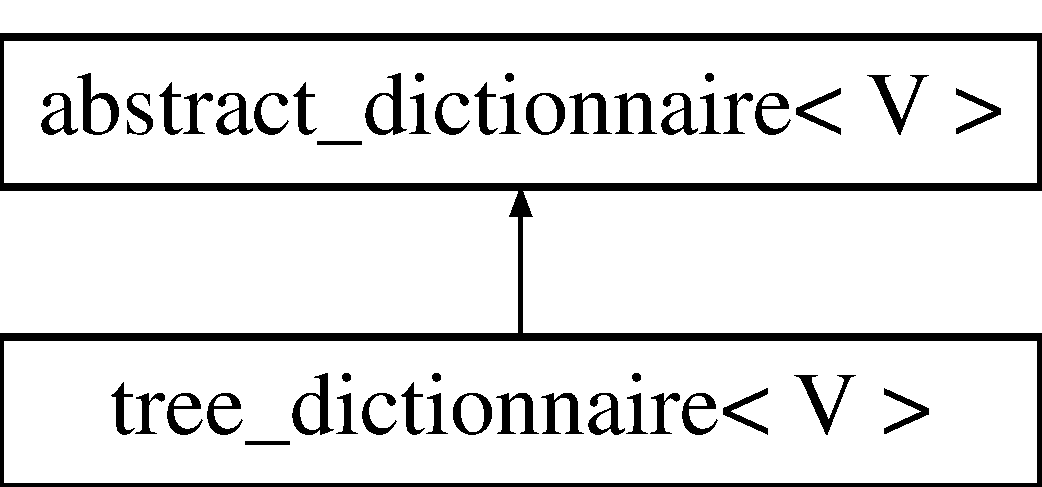
\includegraphics[height=2.000000cm]{classtree__dictionnaire}
\end{center}
\end{figure}
\subsection*{Fonctions membres publiques}
\begin{DoxyCompactItemize}
\item 
ostream \& \hyperlink{classtree__dictionnaire_af8386fa4ca1a5d86ca73d2e1f7845999}{afficher} (ostream \&os=cout) const 
\begin{DoxyCompactList}\small\item\em Affiche le dictionnaire sur le flux passé en paramètre. O(n) \end{DoxyCompactList}\item 
bool \hyperlink{classtree__dictionnaire_a688203a2da7bbc1bdb667868ef6e18a3}{contient\-Mot} (const string \&mot) const 
\begin{DoxyCompactList}\small\item\em Teste si le dictionnaire contient un mot. O(log(n)) \end{DoxyCompactList}\item 
void \hyperlink{classtree__dictionnaire_a867e2a62ee1defe00f00c08e170192d1}{ajouter\-Mot} (const string \&mot, const V \&v)
\begin{DoxyCompactList}\small\item\em Ajoute la chaîne mot au dictionnaire, avec la valeur v, mot étant supposé absent du dictionnaire. O(log(n)) \end{DoxyCompactList}\item 
void \hyperlink{classtree__dictionnaire_afc52a48eea27916d31c7088813e83fd0}{associer\-Mot} (const string \&mot, const V \&v)
\begin{DoxyCompactList}\small\item\em Associe la valeur v à la chaîne mot dans le dictionnaire, mot pouvant être présent ou absent du dictionnaire. O(log(n)) \end{DoxyCompactList}\item 
void \hyperlink{classtree__dictionnaire_a76fa52ac010b861d437b87d1b68fe0cc}{supprimer\-Mot} (const string \&mot)
\begin{DoxyCompactList}\small\item\em Supprime l'éventuelle chaîne mot du dictionnaire. O(log(n)) \end{DoxyCompactList}\item 
V \hyperlink{classtree__dictionnaire_a7fb5e78b2bf0d5e75c9aebb870d43879}{valeur\-Associee} (const string \&mot) const 
\begin{DoxyCompactList}\small\item\em Donne la valeur correspondant à la chaîne mot (supposée figurer dans le dictionnaire). O(log(n)) \end{DoxyCompactList}\item 
\hyperlink{structtriplet}{triplet}$<$ string $\ast$, V $\ast$, int $>$ \hyperlink{classtree__dictionnaire_a1a5c6cd5954ceac7adbd09eb390f610c}{to\-\_\-array} () const 
\begin{DoxyCompactList}\small\item\em Retourne un triplet contenant le tableau des mots du dictionnaire, le tableau des valeurs associées aux mots et la taille de ces tableaux. O(n) \end{DoxyCompactList}\item 
void \hyperlink{classtree__dictionnaire_a5e251a8b18b85bf416729ddde96242b6}{to\-\_\-list} (list$<$ pair$<$ string, V $>$ $>$ \&ls) const 
\begin{DoxyCompactList}\small\item\em Charge les mots et les valeurs du dictionnaire dans la liste passée en paramètre. O(n) \end{DoxyCompactList}\end{DoxyCompactItemize}
\subsection*{Attributs protégés}
\begin{DoxyCompactItemize}
\item 
\hypertarget{classtree__dictionnaire_a6b4a30e7db9751d74526dd3569679b99}{\hyperlink{classnode}{node}$<$ V $>$ {\bfseries \-\_\-root}}\label{classtree__dictionnaire_a6b4a30e7db9751d74526dd3569679b99}

\end{DoxyCompactItemize}


\subsection{Description détaillée}
\subsubsection*{template$<$typename V$>$class tree\-\_\-dictionnaire$<$ V $>$}

Classe \hyperlink{classtree__dictionnaire}{tree\-\_\-dictionnaire} implémente la classe abstraite \hyperlink{classabstract__dictionnaire}{abstract\-\_\-dictionnaire} avec un arbre. V le type des valeurs associées aux mots. 

\subsection{Documentation des fonctions membres}
\hypertarget{classtree__dictionnaire_af8386fa4ca1a5d86ca73d2e1f7845999}{\index{tree\-\_\-dictionnaire@{tree\-\_\-dictionnaire}!afficher@{afficher}}
\index{afficher@{afficher}!tree_dictionnaire@{tree\-\_\-dictionnaire}}
\subsubsection[{afficher}]{\setlength{\rightskip}{0pt plus 5cm}template$<$typename V $>$ ostream \& {\bf tree\-\_\-dictionnaire}$<$ V $>$\-::afficher (
\begin{DoxyParamCaption}
\item[{ostream \&}]{os = {\ttfamily cout}}
\end{DoxyParamCaption}
) const\hspace{0.3cm}{\ttfamily [virtual]}}}\label{classtree__dictionnaire_af8386fa4ca1a5d86ca73d2e1f7845999}


Affiche le dictionnaire sur le flux passé en paramètre. O(n) 


\begin{DoxyParams}{Paramètres}
{\em os} & \-: le flux de sortie \\
\hline
\end{DoxyParams}
\begin{DoxyReturn}{Renvoie}
le flux de sortie 
\end{DoxyReturn}


Implémente \hyperlink{classabstract__dictionnaire_ae472681c840b81cfc512b47dc664774c}{abstract\-\_\-dictionnaire$<$ V $>$}.

\hypertarget{classtree__dictionnaire_a867e2a62ee1defe00f00c08e170192d1}{\index{tree\-\_\-dictionnaire@{tree\-\_\-dictionnaire}!ajouter\-Mot@{ajouter\-Mot}}
\index{ajouter\-Mot@{ajouter\-Mot}!tree_dictionnaire@{tree\-\_\-dictionnaire}}
\subsubsection[{ajouter\-Mot}]{\setlength{\rightskip}{0pt plus 5cm}template$<$typename V $>$ void {\bf tree\-\_\-dictionnaire}$<$ V $>$\-::ajouter\-Mot (
\begin{DoxyParamCaption}
\item[{const string \&}]{mot, }
\item[{const V \&}]{v}
\end{DoxyParamCaption}
)\hspace{0.3cm}{\ttfamily [virtual]}}}\label{classtree__dictionnaire_a867e2a62ee1defe00f00c08e170192d1}


Ajoute la chaîne mot au dictionnaire, avec la valeur v, mot étant supposé absent du dictionnaire. O(log(n)) 


\begin{DoxyParams}{Paramètres}
{\em mot} & \-: le mot à ajouter \\
\hline
{\em v} & \-: la valeur associée au mot \\
\hline
\end{DoxyParams}


Implémente \hyperlink{classabstract__dictionnaire_a0c3af73e050ee04b8a14161052c5e636}{abstract\-\_\-dictionnaire$<$ V $>$}.

\hypertarget{classtree__dictionnaire_afc52a48eea27916d31c7088813e83fd0}{\index{tree\-\_\-dictionnaire@{tree\-\_\-dictionnaire}!associer\-Mot@{associer\-Mot}}
\index{associer\-Mot@{associer\-Mot}!tree_dictionnaire@{tree\-\_\-dictionnaire}}
\subsubsection[{associer\-Mot}]{\setlength{\rightskip}{0pt plus 5cm}template$<$typename V $>$ void {\bf tree\-\_\-dictionnaire}$<$ V $>$\-::associer\-Mot (
\begin{DoxyParamCaption}
\item[{const string \&}]{mot, }
\item[{const V \&}]{v}
\end{DoxyParamCaption}
)\hspace{0.3cm}{\ttfamily [virtual]}}}\label{classtree__dictionnaire_afc52a48eea27916d31c7088813e83fd0}


Associe la valeur v à la chaîne mot dans le dictionnaire, mot pouvant être présent ou absent du dictionnaire. O(log(n)) 


\begin{DoxyParams}{Paramètres}
{\em mot} & \-: le mot à modifier \\
\hline
{\em v} & \-: la valeur associée au mot \\
\hline
\end{DoxyParams}


Implémente \hyperlink{classabstract__dictionnaire_a3d19bb8707514928a5f54e73701f0d1c}{abstract\-\_\-dictionnaire$<$ V $>$}.

\hypertarget{classtree__dictionnaire_a688203a2da7bbc1bdb667868ef6e18a3}{\index{tree\-\_\-dictionnaire@{tree\-\_\-dictionnaire}!contient\-Mot@{contient\-Mot}}
\index{contient\-Mot@{contient\-Mot}!tree_dictionnaire@{tree\-\_\-dictionnaire}}
\subsubsection[{contient\-Mot}]{\setlength{\rightskip}{0pt plus 5cm}template$<$typename V $>$ bool {\bf tree\-\_\-dictionnaire}$<$ V $>$\-::contient\-Mot (
\begin{DoxyParamCaption}
\item[{const string \&}]{mot}
\end{DoxyParamCaption}
) const\hspace{0.3cm}{\ttfamily [virtual]}}}\label{classtree__dictionnaire_a688203a2da7bbc1bdb667868ef6e18a3}


Teste si le dictionnaire contient un mot. O(log(n)) 


\begin{DoxyParams}{Paramètres}
{\em mot} & \-: le mot recherché \\
\hline
\end{DoxyParams}
\begin{DoxyReturn}{Renvoie}
vrai si le dictionnaire contient le mot sinon faux 
\end{DoxyReturn}


Implémente \hyperlink{classabstract__dictionnaire_abeb4f33d1600bcf2a6058f7bdae65aaf}{abstract\-\_\-dictionnaire$<$ V $>$}.

\hypertarget{classtree__dictionnaire_a76fa52ac010b861d437b87d1b68fe0cc}{\index{tree\-\_\-dictionnaire@{tree\-\_\-dictionnaire}!supprimer\-Mot@{supprimer\-Mot}}
\index{supprimer\-Mot@{supprimer\-Mot}!tree_dictionnaire@{tree\-\_\-dictionnaire}}
\subsubsection[{supprimer\-Mot}]{\setlength{\rightskip}{0pt plus 5cm}template$<$typename V $>$ void {\bf tree\-\_\-dictionnaire}$<$ V $>$\-::supprimer\-Mot (
\begin{DoxyParamCaption}
\item[{const string \&}]{mot}
\end{DoxyParamCaption}
)\hspace{0.3cm}{\ttfamily [virtual]}}}\label{classtree__dictionnaire_a76fa52ac010b861d437b87d1b68fe0cc}


Supprime l'éventuelle chaîne mot du dictionnaire. O(log(n)) 


\begin{DoxyParams}{Paramètres}
{\em mot} & \-: le mot à supprimer \\
\hline
\end{DoxyParams}


Implémente \hyperlink{classabstract__dictionnaire_a7063c0c484fe9eabecb0ddb268951823}{abstract\-\_\-dictionnaire$<$ V $>$}.

\hypertarget{classtree__dictionnaire_a1a5c6cd5954ceac7adbd09eb390f610c}{\index{tree\-\_\-dictionnaire@{tree\-\_\-dictionnaire}!to\-\_\-array@{to\-\_\-array}}
\index{to\-\_\-array@{to\-\_\-array}!tree_dictionnaire@{tree\-\_\-dictionnaire}}
\subsubsection[{to\-\_\-array}]{\setlength{\rightskip}{0pt plus 5cm}template$<$typename V $>$ {\bf triplet}$<$ string $\ast$, V $\ast$, int $>$ {\bf tree\-\_\-dictionnaire}$<$ V $>$\-::to\-\_\-array (
\begin{DoxyParamCaption}
{}
\end{DoxyParamCaption}
) const\hspace{0.3cm}{\ttfamily [virtual]}}}\label{classtree__dictionnaire_a1a5c6cd5954ceac7adbd09eb390f610c}


Retourne un triplet contenant le tableau des mots du dictionnaire, le tableau des valeurs associées aux mots et la taille de ces tableaux. O(n) 

\begin{DoxyRefDesc}{Obsolète}
\item[\hyperlink{deprecated__deprecated000007}{Obsolète}]utiliser \hyperlink{classtree__dictionnaire_a5e251a8b18b85bf416729ddde96242b6}{to\-\_\-list()} \end{DoxyRefDesc}
\begin{DoxyReturn}{Renvoie}
le triplet mots-\/valeurs-\/taille 
\end{DoxyReturn}


Implémente \hyperlink{classabstract__dictionnaire_a0b04fb9d2062846f5c9bdc8c7742538f}{abstract\-\_\-dictionnaire$<$ V $>$}.

\hypertarget{classtree__dictionnaire_a5e251a8b18b85bf416729ddde96242b6}{\index{tree\-\_\-dictionnaire@{tree\-\_\-dictionnaire}!to\-\_\-list@{to\-\_\-list}}
\index{to\-\_\-list@{to\-\_\-list}!tree_dictionnaire@{tree\-\_\-dictionnaire}}
\subsubsection[{to\-\_\-list}]{\setlength{\rightskip}{0pt plus 5cm}template$<$typename V $>$ void {\bf tree\-\_\-dictionnaire}$<$ V $>$\-::to\-\_\-list (
\begin{DoxyParamCaption}
\item[{list$<$ pair$<$ string, V $>$ $>$ \&}]{ls}
\end{DoxyParamCaption}
) const\hspace{0.3cm}{\ttfamily [virtual]}}}\label{classtree__dictionnaire_a5e251a8b18b85bf416729ddde96242b6}


Charge les mots et les valeurs du dictionnaire dans la liste passée en paramètre. O(n) 


\begin{DoxyParams}{Paramètres}
{\em ls} & \-: la liste où charger les couples mot-\/valeur \\
\hline
\end{DoxyParams}


Implémente \hyperlink{classabstract__dictionnaire_a0bebd25d66714c37c11f53f0797b2ffd}{abstract\-\_\-dictionnaire$<$ V $>$}.

\hypertarget{classtree__dictionnaire_a7fb5e78b2bf0d5e75c9aebb870d43879}{\index{tree\-\_\-dictionnaire@{tree\-\_\-dictionnaire}!valeur\-Associee@{valeur\-Associee}}
\index{valeur\-Associee@{valeur\-Associee}!tree_dictionnaire@{tree\-\_\-dictionnaire}}
\subsubsection[{valeur\-Associee}]{\setlength{\rightskip}{0pt plus 5cm}template$<$typename V $>$ V {\bf tree\-\_\-dictionnaire}$<$ V $>$\-::valeur\-Associee (
\begin{DoxyParamCaption}
\item[{const string \&}]{mot}
\end{DoxyParamCaption}
) const\hspace{0.3cm}{\ttfamily [virtual]}}}\label{classtree__dictionnaire_a7fb5e78b2bf0d5e75c9aebb870d43879}


Donne la valeur correspondant à la chaîne mot (supposée figurer dans le dictionnaire). O(log(n)) 


\begin{DoxyParams}{Paramètres}
{\em mot} & \-: le mot dont on veut récupérer la valeur associée \\
\hline
\end{DoxyParams}
\begin{DoxyReturn}{Renvoie}
la valeur associée au mot 
\end{DoxyReturn}


Implémente \hyperlink{classabstract__dictionnaire_abf2426d66e5499582dc4dc4fe5eeb1c3}{abstract\-\_\-dictionnaire$<$ V $>$}.



La documentation de cette classe a été générée à partir du fichier suivant \-:\begin{DoxyCompactItemize}
\item 
/home/grdx/git/cpp-\/collections/src/\hyperlink{tree__dictionnaire_8hpp}{tree\-\_\-dictionnaire.\-hpp}\end{DoxyCompactItemize}

\hypertarget{structtriplet}{\section{Référence du modèle de la structure triplet$<$ X, Y, Z $>$}
\label{structtriplet}\index{triplet$<$ X, Y, Z $>$@{triplet$<$ X, Y, Z $>$}}
}


Structure générique permettant de stocker trois objets.  




{\ttfamily \#include $<$abstract\-\_\-dictionnaire.\-hpp$>$}

\subsection*{Attributs publics}
\begin{DoxyCompactItemize}
\item 
\hypertarget{structtriplet_abb054078b3a96581bd22fdcf22b2d9e7}{X {\bfseries first}}\label{structtriplet_abb054078b3a96581bd22fdcf22b2d9e7}

\item 
\hypertarget{structtriplet_ade8bc35f71cffcbe505ede6f1ebfe896}{Y {\bfseries second}}\label{structtriplet_ade8bc35f71cffcbe505ede6f1ebfe896}

\item 
\hypertarget{structtriplet_aabb9092bc2924d46ce68912876e12e3c}{Z {\bfseries third}}\label{structtriplet_aabb9092bc2924d46ce68912876e12e3c}

\end{DoxyCompactItemize}


\subsection{Description détaillée}
\subsubsection*{template$<$typename X, typename Y, typename Z$>$struct triplet$<$ X, Y, Z $>$}

Structure générique permettant de stocker trois objets. 

La documentation de cette structure a été générée à partir du fichier suivant \-:\begin{DoxyCompactItemize}
\item 
src/\hyperlink{abstract__dictionnaire_8hpp}{abstract\-\_\-dictionnaire.\-hpp}\end{DoxyCompactItemize}

\chapter{Documentation des fichiers}
\hypertarget{abstract__dictionnaire_8hpp}{\section{Référence du fichier src/abstract\-\_\-dictionnaire.hpp}
\label{abstract__dictionnaire_8hpp}\index{src/abstract\-\_\-dictionnaire.\-hpp@{src/abstract\-\_\-dictionnaire.\-hpp}}
}


Classe abstraite dictionnaire.  


{\ttfamily \#include $<$iostream$>$}\\*
{\ttfamily \#include $<$string$>$}\\*
{\ttfamily \#include $<$list$>$}\\*
\subsection*{Classes}
\begin{DoxyCompactItemize}
\item 
struct \hyperlink{structtriplet}{triplet$<$ X, Y, Z $>$}
\begin{DoxyCompactList}\small\item\em Structure générique permettant de stocker trois objets. \end{DoxyCompactList}\item 
class \hyperlink{classabstract__dictionnaire}{abstract\-\_\-dictionnaire$<$ V $>$}
\begin{DoxyCompactList}\small\item\em Classe abstraite \hyperlink{classabstract__dictionnaire}{abstract\-\_\-dictionnaire}. \end{DoxyCompactList}\end{DoxyCompactItemize}


\subsection{Description détaillée}
Classe abstraite dictionnaire. \begin{DoxyAuthor}{Auteur}
Alexis Giraudet 

Théo Cesbron 
\end{DoxyAuthor}
\begin{DoxyVersion}{Version}
1.\-0 
\end{DoxyVersion}
\begin{DoxyDate}{Date}
24 avril 2014 
\end{DoxyDate}

\hypertarget{hash__dictionnaire_8hpp}{\section{Référence du fichier src/hash\-\_\-dictionnaire.hpp}
\label{hash__dictionnaire_8hpp}\index{src/hash\-\_\-dictionnaire.\-hpp@{src/hash\-\_\-dictionnaire.\-hpp}}
}


Classe \hyperlink{classhash__dictionnaire}{hash\-\_\-dictionnaire}.  


{\ttfamily \#include \char`\"{}abstract\-\_\-dictionnaire.\-hpp\char`\"{}}\\*
{\ttfamily \#include \char`\"{}hash\-\_\-table.\-hpp\char`\"{}}\\*
\subsection*{Classes}
\begin{DoxyCompactItemize}
\item 
class \hyperlink{classhash__dictionnaire}{hash\-\_\-dictionnaire$<$ V, S $>$}
\begin{DoxyCompactList}\small\item\em Classe \hyperlink{classhash__dictionnaire}{hash\-\_\-dictionnaire} implémente la classe abstraite \hyperlink{classabstract__dictionnaire}{abstract\-\_\-dictionnaire} avec une table de hachage. V le type des valeurs associées aux mots. \end{DoxyCompactList}\end{DoxyCompactItemize}


\subsection{Description détaillée}
Classe \hyperlink{classhash__dictionnaire}{hash\-\_\-dictionnaire}. \begin{DoxyAuthor}{Auteur}
Alexis Giraudet 

Théo Cesbron 
\end{DoxyAuthor}
\begin{DoxyVersion}{Version}
1.\-0 
\end{DoxyVersion}
\begin{DoxyDate}{Date}
24 avril 2014 
\end{DoxyDate}

\hypertarget{hash__table_8hpp}{\section{Référence du fichier /home/grdx/git/cpp-\/collections/src/hash\-\_\-table.hpp}
\label{hash__table_8hpp}\index{/home/grdx/git/cpp-\/collections/src/hash\-\_\-table.\-hpp@{/home/grdx/git/cpp-\/collections/src/hash\-\_\-table.\-hpp}}
}


Classe \hyperlink{classhash__table}{hash\-\_\-table}.  


{\ttfamily \#include $<$functional$>$}\\*
{\ttfamily \#include \char`\"{}map.\-hpp\char`\"{}}\\*
\subsection*{Classes}
\begin{DoxyCompactItemize}
\item 
class \hyperlink{classhash__table}{hash\-\_\-table$<$ K, V, S $>$}
\begin{DoxyCompactList}\small\item\em Implémentation générique d'une table de hachage avec taleaux associatifs. K le type des clefs, V le type des valeurs et S le nombre de maps. \end{DoxyCompactList}\end{DoxyCompactItemize}
\subsection*{Fonctions}
\begin{DoxyCompactItemize}
\item 
{\footnotesize template$<$typename K , typename V , int S$>$ }\\std\-::ostream \& \hyperlink{hash__table_8hpp_a1f9d233a4b026853223886f62feb411b}{operator$<$$<$} (std\-::ostream \&os, const \hyperlink{classhash__table}{hash\-\_\-table}$<$ K, V, S $>$ \&ht)
\begin{DoxyCompactList}\small\item\em Surchage de l'opérateur de flux pour afficher la table de hachage. O(n) \end{DoxyCompactList}\end{DoxyCompactItemize}


\subsection{Description détaillée}
Classe \hyperlink{classhash__table}{hash\-\_\-table}. \begin{DoxyAuthor}{Auteur}
Alexis Giraudet 

Théo Cesbron 
\end{DoxyAuthor}
\begin{DoxyVersion}{Version}
1.\-0 
\end{DoxyVersion}
\begin{DoxyDate}{Date}
24 avril 2014 
\end{DoxyDate}


\subsection{Documentation des fonctions}
\hypertarget{hash__table_8hpp_a1f9d233a4b026853223886f62feb411b}{\index{hash\-\_\-table.\-hpp@{hash\-\_\-table.\-hpp}!operator$<$$<$@{operator$<$$<$}}
\index{operator$<$$<$@{operator$<$$<$}!hash_table.hpp@{hash\-\_\-table.\-hpp}}
\subsubsection[{operator$<$$<$}]{\setlength{\rightskip}{0pt plus 5cm}template$<$typename K , typename V , int S$>$ std\-::ostream\& operator$<$$<$ (
\begin{DoxyParamCaption}
\item[{std\-::ostream \&}]{os, }
\item[{const {\bf hash\-\_\-table}$<$ K, V, S $>$ \&}]{ht}
\end{DoxyParamCaption}
)}}\label{hash__table_8hpp_a1f9d233a4b026853223886f62feb411b}


Surchage de l'opérateur de flux pour afficher la table de hachage. O(n) 


\begin{DoxyParams}{Paramètres}
{\em os} & \-: le flux de sortie \\
\hline
{\em ht} & \-: la table de hachage à afficher \\
\hline
\end{DoxyParams}
\begin{DoxyReturn}{Renvoie}
le flux de sortie 
\end{DoxyReturn}

\hypertarget{map_8hpp}{\section{Référence du fichier src/map.hpp}
\label{map_8hpp}\index{src/map.\-hpp@{src/map.\-hpp}}
}


Classe map.  


{\ttfamily \#include $<$iostream$>$}\\*
{\ttfamily \#include $<$exception$>$}\\*
{\ttfamily \#include $<$list$>$}\\*
\subsection*{Classes}
\begin{DoxyCompactItemize}
\item 
class \hyperlink{classmap}{map$<$ K, V $>$}
\begin{DoxyCompactList}\small\item\em Implémentation générique d'un tableau associatif avec double chaînage de couples. K le type des clefs et V le type des valeurs. \end{DoxyCompactList}\item 
struct {\bfseries map$<$ K, V $>$\-::\-\_\-link}
\begin{DoxyCompactList}\small\item\em Structure maillon. \end{DoxyCompactList}\end{DoxyCompactItemize}
\subsection*{Fonctions}
\begin{DoxyCompactItemize}
\item 
{\footnotesize template$<$typename K , typename V $>$ }\\std\-::ostream \& \hyperlink{map_8hpp_a49787ed14d7d296cbb025666ceea04fc}{operator$<$$<$} (std\-::ostream \&os, const \hyperlink{classmap}{map}$<$ K, V $>$ \&m)
\begin{DoxyCompactList}\small\item\em Surchage de l'opérateur de flux pour afficher la map. O(n) \end{DoxyCompactList}\end{DoxyCompactItemize}


\subsection{Description détaillée}
Classe map. \begin{DoxyAuthor}{Auteur}
Alexis Giraudet 

Théo Cesbron 
\end{DoxyAuthor}
\begin{DoxyVersion}{Version}
1.\-0 
\end{DoxyVersion}
\begin{DoxyDate}{Date}
24 avril 2014 
\end{DoxyDate}


\subsection{Documentation des fonctions}
\hypertarget{map_8hpp_a49787ed14d7d296cbb025666ceea04fc}{\index{map.\-hpp@{map.\-hpp}!operator$<$$<$@{operator$<$$<$}}
\index{operator$<$$<$@{operator$<$$<$}!map.hpp@{map.\-hpp}}
\subsubsection[{operator$<$$<$}]{\setlength{\rightskip}{0pt plus 5cm}template$<$typename K , typename V $>$ std\-::ostream\& operator$<$$<$ (
\begin{DoxyParamCaption}
\item[{std\-::ostream \&}]{os, }
\item[{const {\bf map}$<$ K, V $>$ \&}]{m}
\end{DoxyParamCaption}
)}}\label{map_8hpp_a49787ed14d7d296cbb025666ceea04fc}


Surchage de l'opérateur de flux pour afficher la map. O(n) 


\begin{DoxyParams}{Paramètres}
{\em os} & \-: le flux de sortie \\
\hline
{\em m} & \-: la map à afficher \\
\hline
\end{DoxyParams}
\begin{DoxyReturn}{Renvoie}
le flux de sortie 
\end{DoxyReturn}

\hypertarget{node_8hpp}{\section{Référence du fichier /home/grdx/git/cpp-\/collections/src/node.hpp}
\label{node_8hpp}\index{/home/grdx/git/cpp-\/collections/src/node.\-hpp@{/home/grdx/git/cpp-\/collections/src/node.\-hpp}}
}


Classe node.  


{\ttfamily \#include \char`\"{}map.\-hpp\char`\"{}}\\*
\subsection*{Classes}
\begin{DoxyCompactItemize}
\item 
class \hyperlink{classnode}{node$<$ V $>$}
\begin{DoxyCompactList}\small\item\em Implémentation d'un arbre-\/noeud (un arbre est un noeud qui n'a pas de père, la racine). V le type des valeurs. \end{DoxyCompactList}\end{DoxyCompactItemize}
\subsection*{Fonctions}
\begin{DoxyCompactItemize}
\item 
{\footnotesize template$<$typename V $>$ }\\ostream \& \hyperlink{node_8hpp_a78a9c7737f3b3ff98a6c323d633226e0}{operator$<$$<$} (ostream \&os, const \hyperlink{classnode}{node}$<$ V $>$ \&n)
\begin{DoxyCompactList}\small\item\em Surchage de l'opérateur de flux pour afficher le noeud. O(n) \end{DoxyCompactList}\end{DoxyCompactItemize}


\subsection{Description détaillée}
Classe node. \begin{DoxyAuthor}{Auteur}
Alexis Giraudet 

Théo Cesbron 
\end{DoxyAuthor}
\begin{DoxyVersion}{Version}
1.\-0 
\end{DoxyVersion}
\begin{DoxyDate}{Date}
24 avril 2014 
\end{DoxyDate}


\subsection{Documentation des fonctions}
\hypertarget{node_8hpp_a78a9c7737f3b3ff98a6c323d633226e0}{\index{node.\-hpp@{node.\-hpp}!operator$<$$<$@{operator$<$$<$}}
\index{operator$<$$<$@{operator$<$$<$}!node.hpp@{node.\-hpp}}
\subsubsection[{operator$<$$<$}]{\setlength{\rightskip}{0pt plus 5cm}template$<$typename V $>$ ostream\& operator$<$$<$ (
\begin{DoxyParamCaption}
\item[{ostream \&}]{os, }
\item[{const {\bf node}$<$ V $>$ \&}]{n}
\end{DoxyParamCaption}
)}}\label{node_8hpp_a78a9c7737f3b3ff98a6c323d633226e0}


Surchage de l'opérateur de flux pour afficher le noeud. O(n) 


\begin{DoxyParams}{Paramètres}
{\em os} & \-: le flux de sortie \\
\hline
{\em n} & \-: le noeud à afficher \\
\hline
\end{DoxyParams}
\begin{DoxyReturn}{Renvoie}
le flux de sortie 
\end{DoxyReturn}

\hypertarget{parser__dictionnaire_8cpp}{\section{Référence du fichier src/parser\-\_\-dictionnaire.cpp}
\label{parser__dictionnaire_8cpp}\index{src/parser\-\_\-dictionnaire.\-cpp@{src/parser\-\_\-dictionnaire.\-cpp}}
}


Classe \hyperlink{classparser__dictionnaire}{parser\-\_\-dictionnaire}.  


{\ttfamily \#include $<$algorithm$>$}\\*
{\ttfamily \#include $<$fstream$>$}\\*
{\ttfamily \#include \char`\"{}hash\-\_\-dictionnaire.\-hpp\char`\"{}}\\*
{\ttfamily \#include \char`\"{}tree\-\_\-dictionnaire.\-hpp\char`\"{}}\\*
\subsection*{Classes}
\begin{DoxyCompactItemize}
\item 
class \hyperlink{classparser__dictionnaire}{parser\-\_\-dictionnaire}
\begin{DoxyCompactList}\small\item\em Classe permettant de parser un text et charger les mots dans un dictionnaire en fonction de leur fréquence. \end{DoxyCompactList}\end{DoxyCompactItemize}
\subsection*{Énumérations}
\begin{DoxyCompactItemize}
\item 
enum \hyperlink{parser__dictionnaire_8cpp_ad67b09ef02d97f138a9b239b8b124835}{type\-\_\-dictionnaire} \{ {\bfseries H\-A\-S\-H\-\_\-\-D\-I\-C\-T\-I\-O\-N\-N\-A\-I\-R\-E}, 
{\bfseries T\-R\-E\-E\-\_\-\-D\-I\-C\-T\-I\-O\-N\-N\-A\-I\-R\-E}, 
{\bfseries U\-N\-K\-N\-O\-W\-N}
 \}
\begin{DoxyCompactList}\small\item\em Énumération des différents types de dictionnaires disponibles. \end{DoxyCompactList}\end{DoxyCompactItemize}
\subsection*{Fonctions}
\begin{DoxyCompactItemize}
\item 
\hypertarget{parser__dictionnaire_8cpp_a97ee70a8770dc30d06c744b24eb2fcfc}{void \hyperlink{parser__dictionnaire_8cpp_a97ee70a8770dc30d06c744b24eb2fcfc}{help} ()}\label{parser__dictionnaire_8cpp_a97ee70a8770dc30d06c744b24eb2fcfc}

\begin{DoxyCompactList}\small\item\em Affiche l'aide. \end{DoxyCompactList}\item 
\hypertarget{parser__dictionnaire_8cpp_a0ddf1224851353fc92bfbff6f499fa97}{int {\bfseries main} (int argc, char $\ast$argv\mbox{[}$\,$\mbox{]})}\label{parser__dictionnaire_8cpp_a0ddf1224851353fc92bfbff6f499fa97}

\end{DoxyCompactItemize}


\subsection{Description détaillée}
Classe \hyperlink{classparser__dictionnaire}{parser\-\_\-dictionnaire}. \begin{DoxyAuthor}{Auteur}
Alexis Giraudet 

Théo Cesbron 
\end{DoxyAuthor}
\begin{DoxyVersion}{Version}
1.\-0 
\end{DoxyVersion}
\begin{DoxyDate}{Date}
24 avril 2014 
\end{DoxyDate}

\hypertarget{tree__dictionnaire_8hpp}{\section{Référence du fichier /home/grdx/git/cpp-\/collections/src/tree\-\_\-dictionnaire.hpp}
\label{tree__dictionnaire_8hpp}\index{/home/grdx/git/cpp-\/collections/src/tree\-\_\-dictionnaire.\-hpp@{/home/grdx/git/cpp-\/collections/src/tree\-\_\-dictionnaire.\-hpp}}
}


Classe \hyperlink{classtree__dictionnaire}{tree\-\_\-dictionnaire}.  


{\ttfamily \#include \char`\"{}abstract\-\_\-dictionnaire.\-hpp\char`\"{}}\\*
{\ttfamily \#include \char`\"{}node.\-hpp\char`\"{}}\\*
\subsection*{Classes}
\begin{DoxyCompactItemize}
\item 
class \hyperlink{classtree__dictionnaire}{tree\-\_\-dictionnaire$<$ V $>$}
\begin{DoxyCompactList}\small\item\em Classe \hyperlink{classtree__dictionnaire}{tree\-\_\-dictionnaire} implémente la classe abstraite \hyperlink{classabstract__dictionnaire}{abstract\-\_\-dictionnaire} avec un arbre. V le type des valeurs associées aux mots. \end{DoxyCompactList}\end{DoxyCompactItemize}


\subsection{Description détaillée}
Classe \hyperlink{classtree__dictionnaire}{tree\-\_\-dictionnaire}. \begin{DoxyAuthor}{Auteur}
Alexis Giraudet 

Théo Cesbron 
\end{DoxyAuthor}
\begin{DoxyVersion}{Version}
1.\-0 
\end{DoxyVersion}
\begin{DoxyDate}{Date}
24 avril 2014 
\end{DoxyDate}

\printindex
\end{document}
